%----------------------------------------------------------------------------------------
%	PACKAGES AND OTHER DOCUMENT CONFIGURATIONS
%----------------------------------------------------------------------------------------

\documentclass[
12pt, % The default document font size, options: 10pt, 11pt, 12pt
%oneside, % Two side (alternating margins) for binding by default, uncomment to switch to one side
french, % ngerman for German
singlespacing, % Single line spacing, alternatives: onehalfspacing or doublespacing
%draft, % Uncomment to enable draft mode (no pictures, no links, overfull hboxes indicated)
%nolistspacing, % If the document is onehalfspacing or doublespacing, uncomment this to set spacing in lists to single
%liststotoc, % Uncomment to add the list of figures/tables/etc to the table of contents
%toctotoc, % Uncomment to add the main table of contents to the table of contents
%parskip, % Uncomment to add space between paragraphs
%nohyperref, % Uncomment to not load the hyperref package
headsepline, % Uncomment to get a line under the header
%chapterinoneline, % Uncomment to place the chapter title next to the number on one line
consistentlayout, % Uncomment to change the layout of the declaration, abstract and acknowledgements pages to match the default layout
openany
]{MastersDoctoralThesis} % The class file specifying the document structure

\usepackage[utf8]{inputenc} % Required for inputting international characters
\usepackage[T1]{fontenc} % Output font encoding for international characters

\usepackage{mathpazo} % Use the Palatino font by default

\usepackage{algorithm}
\usepackage{algorithmic}
\usepackage{palatino}
\usepackage[backend=bibtex,style=authoryear,natbib=true]{biblatex} % Use the bibtex backend with the authoryear citation style (which resembles APA)

\usepackage[autostyle=true]{csquotes} % Required to generate language-dependent quotes in the bibliography

\usepackage{xcolor,colortbl}

%----------------------------------------------------------------------------------------
%	MARGIN SETTINGS
%----------------------------------------------------------------------------------------

\geometry{
	paper=a4paper, % Change to letterpaper for US letter
	inner=2.2cm, % Inner margin
	outer=2.2cm, % Outer margin
	bindingoffset=.3cm, % Binding offset
	top=1.5cm, % Top margin
	bottom=1.5cm, % Bottom margin
	%showframe, % Uncomment to show how the type block is set on the page
}

%----------------------------------------------------------------------------------------
%	THESIS INFORMATION
%----------------------------------------------------------------------------------------

\thesistitle{Une approche de clustering pour la détection des attaques DoS dans un réseau SDN} % Your thesis title, this is used in the title and abstract, print it elsewhere with \ttitle
\supervisor{Pr. Boughaci} % Your supervisor's name, this is used in the title page, print it elsewhere with \supname
\degree{Master en réseaux et systèmes distribués} % Your degree name, this is used in the title page and abstract, print it elsewhere with \degreename
\author{DRIA \textsc{salim}} % Your name, this is used in the title page and abstract, print it 

\subject{Informatique Sciences} % Your subject area, this is not currently used anywhere in the template, print it elsewhere with \subjectname
\keywords{} % Keywords for your thesis, this is not currently used anywhere in the template, print it elsewhere with \keywordnames
\university{\href{http://www.usthb.dz}{Université des sciences et de la technologie Houari Boumediene}} % Your university's name and URL, this is used in the title page and abstract, print it elsewhere with \univname
\department{\href{http://fei.usthb.dz/}{Département d’Informatique}} % Your department's name and URL, this is used in the title page and abstract, print it elsewhere with \deptname
\faculty{\href{http://https://www.fei.usthb.dz/}{Faculté d’Électronique et d'Informatique}} % Your fac

\AtBeginDocument{
\hypersetup{pdftitle=\ttitle} % Set the PDF's title to your title
\hypersetup{pdfauthor=\authorname} % Set the PDF's author to your name
\hypersetup{pdfkeywords=\keywordnames} % Set the PDF's keywords to your keywords
}

\begin{document}

\pagestyle{plain} % Default to the plain heading style until the thesis style is called for the body content

%----------------------------------------------------------------------------------------
%	TITLE PAGE
%----------------------------------------------------------------------------------------

\begin{titlepage}
\begin{center}

\vspace*{.06\textheight}
{\scshape\LARGE \univname\par}\vspace{1.5cm} % University name
\textsc{\Large Mémoire de Master}\\[0.5cm] % Thesis type

\HRule \\[0.4cm] % Horizontal line
{\huge \bfseries \ttitle\par}\vspace{0.4cm} % Thesis title
\HRule \\[1.5cm] % Horizontal line
 
\begin{minipage}[t]{0.45\textwidth}
\begin{flushleft} \large
\emph{Auteurs:}\\
{\authorname}
\\
{BENCHIKH ELHOCINE \textsc{med reda}}
\end{flushleft}
\end{minipage}
\begin{minipage}[t]{0.45\textwidth}
\begin{flushright} \large
\emph{Superviseur:} \\
{\supname} % Supervisor name - remove the \href bracket to remove the link  
\end{flushright}
\end{minipage}\\[1.5cm]
 
\begin{minipage}[t]{0.5\textwidth}
\begin{flushleft} \large
\emph{Membre du jury:}\\
{BENCHIKH \textsc{med reda}}
\\
{BENCHIKH \textsc{med reda}}
\end{flushleft}
\end{minipage}\\[3cm]

\vfill

\large \textit{Mémoire présentée en vue de l'obtention du diplôme de maîtrise en Réseaux et Systèmes Distribués}\\[0.3cm] % University requirement text
\textit{}\\

{\large \today}\\[4cm] % Date
%\includegraphics{Logo} % University/department logo - uncomment to place it
 
\vfill
\end{center}
\end{titlepage}

%----------------------------------------------------------------------------------------
%	QUOTATION PAGE
%----------------------------------------------------------------------------------------

\vspace*{0.2\textheight}

%\noindent\enquote{\itshape Thanks to my solid academic training, today I can write hundreds of words on virtually any topic without possessing a shred of information, which is how I got a good job in journalism.}\bigbreak

%\hfill DAVE Bary 

%----------------------------------------------------------------------------------------
%	ABSTRACT PAGE
%----------------------------------------------------------------------------------------

%\chapter{Résumé}

Software-defined Networking, ou les réseaux définis par logiciel, en tant que technologie émergente, apportent de l’innovation dans la mise en réseau. Avec le découplage du plan de contrôle et du plan de données, le SDN offre une architecture  réseau programmable. En raison des avantages que apporte cette architecture, de nombreuses entreprises sont passées de l’architecture réseau traditionnelle à la nouvelle architecture SDN. Cependant, SDN comme une nouvelle technologie a surgi plusieurs questions qui posent un défi à son avenir. La sécurité est l’un des principaux enjeux qui menace le SDN. Les attaques par déni de service est une forme de menace à laquelle les réseaux SDN sont les plus exposés et les dégats qui peuvent surgir à l’occurence de ces attaques sont clolosales.\\

\noindent Ce travail vise à apporter une solution pour la détection des attaques par déni de service au sein d’un réseau SDN. Nous avons développé, au cours de ce travail, un système de détection d’attaque DoS composé de deux modules ; un qui capture et analyse le flux de trafic et le deuxième identifie la nature de chaque flux capturé (flux bénin ou attaques) en utilisant une approche de clustering. 

%----------------------------------------------------------------------------------------
%	LIST OF CONTENTS/FIGURES/TABLES PAGES
%----------------------------------------------------------------------------------------
\setcounter{tocdepth}{2}
\frontmatter

\tableofcontents % Prints the main table of contents

\listoffigures % Prints the list of figures

\listoftables % Prints the list of tables

%----------------------------------------------------------------------------------------
%	THESIS CONTENT - CHAPTERS
%----------------------------------------------------------------------------------------

 % Begin numeric (1,2,3...) page numbering

\pagestyle{thesis} % Return the page headers back to the "thesis" style

% Include the chapters of the thesis as separate files from the Chapters folder
% Uncomment the lines as you write the chapters


\chapter{Liste des abréviations} 
\label{Abbreviation}

\begin{tabular}{ m{2cm} m{8cm} }
\textbf{SDN} & \textbf{S}oftware \textbf{D}efined \textbf{N}etworking\\

\textbf{API} & \textbf{A}pplication \textbf{P}rogramming \textbf{I}nterface\\

\textbf{ONF} & \textbf{O}pen \textbf{N}etworking \textbf{F}oundation\\

\textbf{OF} & \textbf{O}pen \textbf{F}low\\

\textbf{IDS} & \textbf{I}ntrusion \textbf{D}etection \textbf{S}ystem\\

\textbf{IPS} & \textbf{I}ntrusion \textbf{P}revention \textbf{S}ystem\\

\textbf{DoS} & \textbf{D}enial \textbf{O}f \textbf{S}ervice attack \\

\textbf{NIDS} & \textbf{N}etwork \textbf{I}ntrusion \textbf{D}etection \textbf{S}ystem\\

\textbf{HIDS} & \textbf{H}ost \textbf{I}ntrusion \textbf{D}etection \textbf{S}ystem\\

\textbf{SVM} & \textbf{S}upport \textbf{V}ector \textbf{M}achine \\
\end{tabular}

\chapter{Introduction générale} 

\label{Introduction} 
Durant ces deux dernières décennies les technologies de l’information ont  énormément évolué et leur domaine d’application est de plus en plus vaste. L’internet est utilisée dans tous les secteurs, industrie, éducation, commerce,...etc. La demande des services Cloud augmente considérablement et les gens utilisent de plus en plus les réseaux sociaux. Malheureusement les réseaux traditionnels ne sont pas adéquat à ces nouvelles technologies de l’information  pour plusieurs raisons, par exemple; leur scalabilité limitée, ils consomment trop de ressources matériels,  leur structure est complexe, ils sont aussi coûteux et difficiles à gérer.  Ce qui oblige à concevoir des réseaux évolutifs, fiables et robustes pour faire face à ces problèmes.\\

	Comme solution la technologie Software Defined Networking a été proposée, son but est de rendre les réseaux programmables par logiciel contrairement aux réseaux traditionnels qui nécessitaient l’intervention humaine  pour configurer chaque équipement à part qui est une opération fastidieuse, prend beaucoup de temps et exposé aux erreurs de configuration. Le SDN rend ce concept de réseau programmable possible en introduisant un nouvel équipement dit contrôleur, ce dernier va être le cerveau du réseau, toute décision liée au routage du trafic réseau, la sécurité, la gestion des équipements est prise par le contrôleur.\\
	
	Cependant cette technologie souffre de nombreux problèmes de sécurité certains sont hérités de l’environnement réseau, tandis que d’autre sont propre à l’architecture SDN. La nature centralisée de l’architecture SDN est exploitée pour mener des attaques contre le contrôleur, une fois compromis, l’attaquant aura un contrôle total du réseau, il peut reconfigurer les équipements, rediriger le trafic réseau ailleurs, lancer d’autre attaques. Donc il est essentiel de bien sécuriser l'architecture SDN, spécialement le contrôleur, pour garantir le bon fonctionnement du réseau.\\
	
	Le travail qui nous a été confié est de concevoir un système de détection des attaques par déni de service (DoS) dans un réseau SDN. L’apprentissage automatique, plus précisément, le Clustering, sera la méthode adoptée pour concevoir ce système. Ce système doit écouter les messages échangés dans le réseau et il doit être capable de détecter tout attaque de type DoS en extrayant les informations des flux qui permettent  de spécifier la nature du flux, dire quoi faire lors de l’occurrence d’une attaque et apprendre de nouveaux motifs. Chaque attaque DoS a un motif précis il peut être  le nombre de paquets envoyés, l’intervalle de temps entre deux paquets consécutifs, la durée de l’attaque, la taille moyenne des paquets, ...etc.\\
\newpage
Afin de bien mener le travail dans le cadre approprié, ce mémoire est structuré comme suit; Dans un premier lieu, nous commençons par définir le concept des réseaux programmables par logiciel, voir les avantages et les inconvénients qu'apporte cette nouvelle technologie, nous passerons par la suite à la sécurité des réseaux SDN où nous étudierons en détail l'aspect sécurité des réseaux, nous verrons les majeures contraintes de sécurités qui doivent être respectées pour garantir le bon fonctionnement du SDN, les différents type d’attaques auxquels un environnement SDN est exposé et une étude comparative entre des travaux existants dans le même contexte que notre travail. Nous entamerons ensuite la conception en commençant par l'analyse et la spécification des besoins pour passer à la modélisation du système en décrivant son architecture générale et les différents modules qui le composent. Une fois notre système réalisé, il ne reste que le mettre sous le test pour évaluer ces performances et son efficacités dans un réseau SDN simulé. La dernière section de ce mémoire sera une conclusion générale sur le travail que nous allons faire.\\
 
\mainmatter
% Chapter 1
\mainmatter
\chapter{Software Defined Networking} 

\label{Chapter1} 

Les nouvelles exigences des réseaux modernes en terme d’adaptabilité, d’automatisation, de maintenabilité ont fait naître une nouvelle technologie de réseaux informatique, connue sous le nom de \textit{Software Defined Networking}, qui donne un contrôle centralisé et programmable des ressources réseaux.\\
Ce chapitre donne un aperçu sur l’environnement SDN et montre comment il est conçu  pour répondre aux besoins changeants du réseau.
%----------------------------------------------------------------------------------------

\section{Limites des réseaux traditionnelles}
Avant de passer au Software-Defined Networking, rappelons deux majeures limites des réseaux traditionnels cités par l'ONF (Open Networking Foundation) [\cite{1}] :\\
\begin{itemize}
\item[•] \textbf{Architecture statique et complexe} : pour répondre aux différents niveaux de qualité de service, le volume de trafic élevé et les exigences en matière de sécurité; la technologie réseau est devenue plus complexe et difficile à gérer. Cela a donné lieu à un certain nombre de protocoles définis de façon indépendante dont chacun répond à une partie des besoins de réseautage. Un exemple de la difficulté que cela présente est lorsque les appareils sont ajoutés ou déplacés. Le personnel de gestion du réseau doit utiliser des outils de gestion au niveau de l’appareil pour modifications des paramètres de configuration dans plusieurs commutateurs, routeurs, pare-feu,...etc. Les opérations de mise à jour sont fastidieuses et coûteuses en matière de temps et donnent place aux erreurs de configuration qui peuvent engendrer des problèmes au niveau du réseau.\\
\item[•] \textbf{Scalabilité limitée} : la demande sur les réseaux augmente rapidement, tant en volume qu’en variétés. Ajouter plus de commutateurs ou augmenter la capacité de transmission est difficile en raison de la complexité et nature statique du réseau.
\end{itemize}

%----------------------------------------------------------------------------------------
\newpage
\section{Une approche réseau moderne}
Une approche réseau moderne doit satisfaire les exigences citées par L’Open Data Center Alliance (ODCA)  [\cite{2}], notamment :\\
\begin{itemize}
\item[•] \textbf{Adaptabilité}: les réseaux doivent s’adapter dynamiquement, en fonction des besoins des applications, des activités, la politique et les conditions du réseau.\\
\item[•] \textbf{Automatisation}: les changements de politique doivent être propagé automatiquement afin de réduire le travail manuel et les erreurs.\\
\item[•] \textbf{Sécurité intégrée}: les applications réseau doivent intégrer la sécurité comme service de base et non pas comme solution complémentaire.\\
\item[•] \textbf{Mise à l’échelle sur demande}: les implémentations doivent avoir la capacité à prendre de l’expansion ou à réduire le réseau et ses services pour répondre aux requêtes à la demande.
\end{itemize}

%----------------------------------------------------------------------------------------

\section{Définition}

Software-defined networking est une nouvelle architecture réseau, qui a pour but pratique de rendre programmables les réseaux par le biais d’un contrôleur centralisé. Rappelons que dans les réseaux traditionnels les périphériques réseaux (commutateurs et routeurs) construisent leurs tables de routage localement, ce qui signifie qu’ils prennent leurs propres décisions en interne sur la meilleure façon d’aiguiller le trafic. \\

Dans les SDN les décisions de routage sont prises par un contrôleur centralisé ce qui fait que les périphériques n’ont plus intérêt à prendre des décisions localement, ils n’ont qu’à suivre celles prises par le contrôleur. Ce qui rend cette architecture dynamique, programmable et idéale pour les réseaux modernes à haute demande.

%----------------------------------------------------------------------------------------

\section{Architecture SDN}

Le concept central derrière l’architecture SDN est de permettre aux développeurs et gestionnaires de réseau d’avoir un contrôle centralisé sur les équipements réseau.\\

Le SDN fait la séparation entre le plan de contrôle et le plan de données. Le plan de contrôle est responsable des décisions de transmission, il comprend des mécanismes de transmission d’itinéraire du trafic. Le plan de données représente la partie des commutateurs et routeurs qui assurent effectivement la transmission des données. La différence entre l’architecture traditionnelle  et l’architecture SDN est illustrée dans la figure suivante:

\newpage
\begin{figure}[h]
\centering
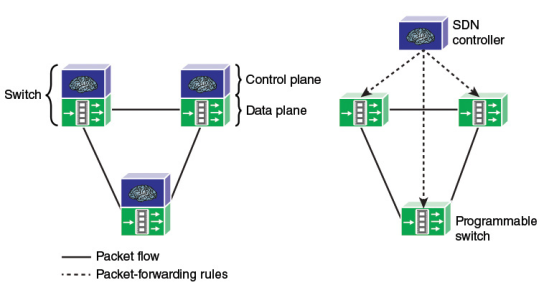
\includegraphics[width=0.7\textwidth]{Figures/SDN_Architecture}
\decoRule
\caption{Plan de données et plan de contrôle}
\label{fig:SDN_Architecture}
\end{figure}

Dans l’architecture traditionnelle le plan de données et le plan de contrôle sont intégrés dans un même équipement physique. Par contre dans Le SDN le plan de contrôle est externalisé de tous les périphériques réseaux et associé à un équipement dit contrôleur.

\begin{figure}[h]
\centering
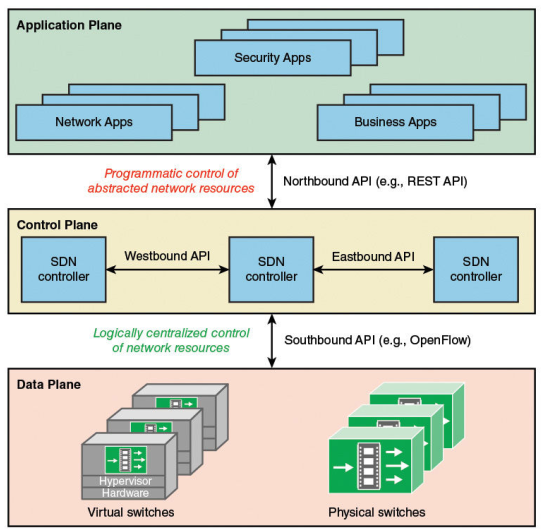
\includegraphics[width=0.55\textwidth]{Figures/SDN_Plans}
\decoRule
\caption{Architecture SDN}
\label{fig:SDN_Plans}
\end{figure}

L’architecture SDN définit trois couches,  comme indiqué dans la figure \ref{fig:SDN_Plans}, chacune représente un plan, plan de données, plan de contrôle ou plan d’application. Chaque couche ne peut communiquer qu’avec ces couches voisines. 

\subsection{Plan de Données}
Le plan de données se compose de commutateurs physiques et de commutateurs virtuels, qui sont responsables de la transmission des paquets. Cependant chaque commutateur doit implémenter un modèle de transfert de paquet, ce modèle est défini à travers une API (Application programming interface) qui réside entre le plan de contrôle et le plan de données permettant la communication entre le contrôleur et les commutateurs du plan de données. Parmi ces API, le OpenFlow, qui nous allons détailler par la suite.\\

\noindent Le plan de données assure une fonction autre que la transmission des données, le support de contrôle. Cette fonction permet la communication avec le contrôleur SDN pour l’échange des informations liées à la gestion du périphérique.  
%----------------------------------------------------------------------------------------

\subsection{Plan de Contrôle}
Le plan de contrôle SDN, composé d’un ou plusieurs contrôleurs, mappe les demandes de service de couche d’application en commandes et directives spécifiques aux commutateurs du plan de données et fournit aux applications des informations sur la topologie et l’activité du plan de données.\\

\noindent Le contrôleur définit les flux de données qui se produisent dans le plan de données. Un flux est une séquence de paquets qui partagent un ensemble de valeurs de champ d'en-tête. Pour qu’un flux traverse le réseau, le contrôleur intervient pour vérifier si ce flux est autorisé dans le cadre de la politique réseau définie.\\

\noindent Dans ce qui suit, trois frameworks les plus utilisés pour la mise en œuvre des contrôleurs SDN:\\
\begin{itemize}
\item[]\textbf{OpenDaylight}[\cite{3}]: Un framework open source, écrit en java, permettant la programmation réseau. OpenDaylight a été développé par Cisco et IBM, il permet à plusieurs contrôleurs distribués, résidants dans des serveurs différents, de fonctionner comme étant un seul contrôleur centralisé.\\
\item[]\textbf{Ryu}[\cite{4}]: Framework open source développé par NTT labs, basé composant et entièrement écrit en python. Ryu fournit des composants logiciels avec API bien définie qui rend la tâche facile aux développeurs pour créer de nouvelles applications de gestion et de contrôle.\\
\item[]\textbf{NOX}[\cite{5}]: Développé par Nicira networks, NOX est une plateforme conçue spécialement pour le développement des applications de contrôle de réseau.
\end{itemize} 

\newpage
\subsection{Plan d'Applications}
Le plan d’application contient des applications et des services qui définissent, surveillent et contrôlent les ressources et le comportement du réseau. Ces applications interagissent avec le plan de contrôle via des interfaces dédiées pour que la couche de contrôle personnalise automatiquement le comportement et les propriétés des ressources réseau. La programmation d’une application SDN utilise la vue abstraite des ressources réseau fournie par la couche de contrôle au moyen d’informations et de modèles de données exposés via l’API fournie.
%----------------------------------------------------------------------------------------

\section{Caractéristiques des SDN}
Après avoir vu la nouvelle architecture réseau, le software-defined Networking, en opposition avec l'architecture traditionnelle,nous trouvons que les principales caractéristiques des SDN sont les suivantes :\\
\begin{itemize}
\item[-]\textbf{Séparation des plans}: le plan de contrôle est séparé du plan de données. Les périphériques de plan de données deviennent des simples dispositifs de transfert de paquets. Le plan de contrôle est installé dans un contrôleur ou ensemble de contrôleurs centralisés et coordonnés.\\
\item[-]\textbf{Programmabilité}: le réseau est programmable par des applications qui s’exécutent au-dessus du contrôleur SDN. Les contrôleurs présentent une vue abstraite des ressources du réseau aux applications.\\
\item[-]\textbf{Centralisation}: le cerveau du réseau est (logiquement) centralisée dans des contrôleurs SDN basé sur des logiciels qui maintiennent une vue globale du réseau.
\end{itemize}

%----------------------------------------------------------------------------------------
\section{OpenFlow et SDN}
\label{S_OpenFlow}
Pour implémenter le concept SDN en pratique, un protocole standardisé et sécurisé est essentiel  pour établir la connexion entre le contrôleur et les ressources réseau. L’architecture Openflow se compose de trois éléments principaux: un commutateur Openflow, un contrôleur externe et le protocole Openflow. Le plan de données et le plan de contrôle communiquent sur un canal sécurisé via ce protocole. Le commutateur Openflow dispose de tables de flux et d’une couche d’abstraction qui communique en toute sécurité avec un contrôleur via le protocole Openflow. La table de flux contient des entrées de flux qui déterminent comment les paquets appartenant à un flux seront traités et transmis. 
Les entrées de flux consistent en :\\

\begin{itemize}
\item[•] Matching rules – pour apparier les paquets entrants.
\item[•] Counters – pour collecter des statistiques du flux.
\item[•] Set of instructions / actions - à appliquer en cas de correspondance.\\
\end{itemize}

Lorsqu’un paquet arrive à un commutateur Open Flow, les champs d’en-tête du paquet sont extraits et comparés aux règles correspondances. Si une correspondance est trouvée, le commutateur applique l’action appropriée. S’il n’y a pas de correspondance, l’action effectuée par le commutateur dépend de l’instruction définie par l’entrée de \textit{ table-miss flow}. Chaque table de flux doit avoir cette entrée afin de gérer la non-correspondance d’un flux dans une table. Des exemples d’actions qui peuvent être effectuées lorsque'aucune correspondance n’est trouvée sont: abandonner le paquet, continuer le processus de correspondance sur la table de flux suivant, acheminer le paquet au contrôleur. 

\subsection{Table de Flux}
La table de flux contient plusieurs entrées. Chaque entrée de cette table a la structure suivante:\\
\begin{table}[h]
\begin{center}
\begin{tabular}{ | c | c | c | c | c | c |}
\hline
\rowcolor[rgb]{0.85,0.85,0.85}
Match Fields & Priority & Counters & Instructions & Timeouts & Cookie\\
\hline
\end{tabular}
\caption{Entrée d'une table de flux}
\end{center}
\end{table}
\begin{itemize}

\item[-]\textbf{Match Fields}: permet de sélectionner des paquets qui correspondent aux valeurs des champs de Match Fields.
\item[-]\textbf{Priority}: un champ sur 16 bits, définit la priorité de l'entrée. la valeur O correspond à la priorité la plus basse.
\item[-]\textbf{Counters}: un conteur de paquets. Il est mis à jour lors d'une correspondance d'un paquet à une entrée de la table de flux. 
\item[-]\textbf{Instructions}: ensemble d'instructions à déclencher en cas de correspondance. 
\item[-]\textbf{Timeouts}: durée de vie d'une entrée de table.
\item[-]\textbf{Cookie}: utilisé par le contrôleur pour le filtrage de paquets.\\
\end{itemize}

Le champ principal dans une entrée de table de flux est le \textbf{Match Fields}, ce dernier définit un vecteur d'attributs correspondant aux champs de l’entête du paquet arrivé au commutateur.\\

\begin{table}[h]
\begin{center}
\begin{tabular}{ | m{0.7cm} | m{0.7cm} | m{0.7cm} | m{0.7cm} | m{0.7cm} | m{0.7cm} | m{0.7cm} | m{0.7cm} | m{0.7cm} | m{0.7cm} | m{0.7cm} | m{0.7cm} | m{0.7cm} | m{0.7cm} |}
\hline
\rowcolor[rgb]{0.80,0.80,0.80}
 Port Ent & Port Srt & Ethr AS & Ethr AD & Ethr Type & IP & AS IPv4 & AD IPv4 & AS IPv6 & AD IPv6 & TCP Src & TCP Dest & UDP Src & UDP Dest\\
\hline
\end{tabular}
\caption{Match Fields}
\end{center}
\end{table}

\begin{itemize}
\item[\textbf{Port Ent}]: Identificateur du port par lequel le paquet est arrivé.
\item[\textbf{Port Srt}]: Identificateur du port de sortie.
\item[\textbf{Ethr AS et Ethr AD}]: Adresses Ethernet, source et destination. 
\item[\textbf{Ethr Type}]: Type de trame Ethernet.
\item[\textbf{IP Type}]: version IP, 4 ou 6
\item[\textbf{AS IPv4 et AD IPv4}]: Adresses IPv4, source et destination.
\item[\textbf{AS IPv6 et AD IPv6}]: Adresses TPv6, source et destination.
\item[\textbf{TCP Src et TCP Dest, UDP Src et UDP Dest}]: Ports source et destination de couche de transport.
\end{itemize}

%----------------------------------------------------------------------------------------
\newpage
\section{Contrôleur SDN}
Comme mentionné précédemment, le contrôleur est le composant principal de toute l'infrastructure SDN où tous les calculs y sont effectués. Il est responsable de la gestion de tout le réseau.\\
En résumé, les fonctions assurées par un contrôleur SDN sont [\cite{6}]: \\

\noindent\textbf{- Routage plus court chemin}: utilise les informations de routage collectées à partir des commutateurs pour établir la table de routage.\\
\textbf{- Gestion de notifications}: reçoit, traite et transmet à un événement d’application, les notifications d’alarme, les alarmes de sécurité et les changements d’état.\\
\textbf{- Sécurité}: fournit des services de sécurité.\\
\textbf{- Gestion de topologie}: construit et maintient les informations sur l'interconnexion des équipements réseau.\\
\textbf{- Gestion de statistique}: collecte et stock des informations sur le trafic réseau.\\
\textbf{- Gestion de périphériques}: configure les paramètres des commutateurs et gère les tables de flux \autoref{S_OpenFlow}.
 

\section{Avantages et inconvénients des SDN}
\subsection{Avantages}
\noindent - Économies opérationnelles: les SDN réduisent les dépenses d’exploitation. Les services de réseau peuvent être gérés par des applications, libérant ainsi l’équipe de réseautage.\\

\noindent - Une meilleure gestion: les SDN offrent une gestion centralisée et automatisée des équipements réseau.\\

\noindent - Flexibilité: les SDN créent une flexibilité dans la façon dont le réseau peut être exploité. Les administrateurs réseau peuvent écrire leurs propres services de réseau en utilisant les outils de développement standard.\\

\noindent - Disponibilité améliorée: en éliminant l’intervention manuelle, les SDN permettent de réduire les erreurs de configuration et de déploiement qui peuvent affecter le réseau. 

\subsection{Inconvénients}
\noindent - Il faut modifier entièrement l’infrastructure réseau  pour mettre en œuvre le SDN. Il faut donc reconfigurer complètement le réseau. Cela implique des dépenses considérables en vue de mettre en œuvre cette technologie.\\

\noindent- SDN à ses propres vulnérabilités de sécurité. Ceci nécessite de mettre en place de nouvelles approches pour veiller sur la sécurité du réseau.\\

\noindent- Toute l'intelligence du réseau est placée dans le contrôleur, ce qui constitue un point de défaillance unique. Si le contrôleur tombe en panne ou il est compromis tout le réseau cessera de fonctionner.

\section{Conclusion}
Le Software Defined Networking annonce des changements importants sur les réseaux dans les années à venir. Ce chapitre n'a parlé que brièvement sur cette nouvelle technologie, sa définition est bien plus vague et son domaine d'application est bien plus large. Les profits qui peuvent être tirés de cette technologie sont innombrables si bien exploitée.

% Chapter 2
\chapter{Sécurité des réseaux}

\label{Chapter2} 

Les réseaux définis par logiciel sont une catégorie émergente de réseaux qui présente de nouveaux défis du point de vue sécurité. Ce chapitre fournit un aperçu complet sur les menaces de sécurité auxquelles est confrontée cette architecture émergente, en particulier les attaques par déni de service DoS. Différentes solutions déjà proposées pour sécuriser cette technologie vont être vues et examinées au cours de ce chapitre afin de mieux comprendre comment l'aspect de sécurité est géré au sein d'un réseau SDN; ce qui nous aidera par la suite à proposer une solution adéquate pour la détection des attaques DoS dans un tel réseau.

\section{Sécurité dans un réseau Informatique}

\subsection{Généralités}
La sécurité des réseaux informatiques est la stratégie et les dispositions d’une organisation pour assurer la sécurité de ses actifs et de tout le trafic réseau. Elle se manifeste par une mise en œuvre des mécanismes qui sont conçus pour détecter, prévenir et lutter contre une attaque de sécurité et des services de sécurité qui augmentent celle des traitements et des échanges de données d’un système. Un service de sécurité utilise un ou plusieurs mécanismes de sécurité.\\

\noindent Lors du développement d’un réseau sécurisé, il convient de prendre en compte les services suivants:\\
\begin{itemize}
\item[•]\textbf{L’authenticité}: l’identité des acteurs de la communication est vérifiée.\\
\item[•]\textbf{La confidentialité}: les données (et l'objet et les acteurs) de la communication ne peuvent pas être connues d’un tiers non autorisé.\\
\item[•]\textbf{L’intégrité}: les données de la communication n’ont pas été altérées.\\
\item[•]\textbf{La disponibilité}: les acteurs de la communication accèdent aux données dans de bonnes conditions.\\
\item[•]\textbf{La non-répudiation}: les acteurs impliqués dans la communication ne peuvent nier y avoir participé.
\end{itemize}

\newpage

\subsection{Les menaces d’un réseau informatique}
Une attaque est une action qui compromet la sécurité des informations. Les attaques peuvent être classées en deux catégories:\\
\begin{itemize}
\item[\textbf{Attaque passive}]: consiste à écouter sans modifier les données ou le fonctionnement du réseau. Elle est généralement indétectable mais une prévention est possible.\\
\item[\textbf{Attaque active}]: consiste à modifier des données ou des messages, à s'introduire dans des équipements réseau ou à perturber le bon fonctionnement de ce réseau. Noter qu'une attaque active peut être exécutée sans la capacité d'écoute.
\end{itemize}

\subsection{Les mécanismes de sécurité}
\begin{itemize}
\item[•]\textbf{Pare-feu}: un élément (logiciel ou matériel) du réseau informatique contrôlant les communications qui le traversent. Il a pour fonction de faire respecter la politique de sécurité du réseau, celle-ci définissant les communications autorisées ou interdites. Il n'empêche pas un attaquant d'utiliser une connexion autorisée pour attaquer le système. Il ne protège pas contre une attaque venant du réseau intérieur (qui ne le traverse pas).\\
\item[•]\textbf{Antivirus}: logiciel sensé protéger l'ordinateur contre les logiciels (ou fichiers potentiellement exécutables) néfastes. Il ne protège pas contre un intrus qui emploie un logiciel légitime, ou contre un utilisateur légitime qui accède à une ressource alors qu'il n'est pas autorisé à le faire.\\
\item[•]\textbf{Détection d'intrusion}: repère les activités anormales ou suspectes sur le réseau surveillé, ne détecte pas les accès incorrects mais autorisés par un utilisateur légitime. Mauvaise détection : taux de faux positifs, faux négatifs.\\
\item[•]\textbf{Contrôle d’accès}: vérifie les droits d’accès d'un acteur aux données, n'empêche pas l'exploitation d'une vulnérabilité.
\end{itemize}

\section{La sécurité dans les réseaux SDN}
Le but des SDN est de rendre les réseaux informatiques plus sécurisés et robustes. La gestion centralisée des SDN simplifie la façon dont les mécanismes de sécurité sont introduits dans le réseau. Cependant cette solution ouvre les porte à d'autres types d'attaque : attaques initiées à partir des applications de gestion malicieuses, attaques sur le contrôleur, infecter les switches.\\\\
Selon Kreutz et al[\cite{7}], les vecteurs d'attaques identifiés dans les SDN sont décrits dans le tableau \ref{table:Threat_Vectors}.
\newpage
\begin{table}[h]
\begin{center}
\begin{tabular}{  m{0.5cm} m{11cm} }
\hline
\textbf{N}. & \textbf{Vecteur d'attaque}\\
\hline
1 & Flux de trafic falsifié ou truqué\\
2 & Attaques contre les vulnérabilités des commutateurs\\
3 & Attaque sur les liens de communication du contrôleur\\
4 & Attaques contre les vulnérabilités des contrôleurs\\
5 & Manque de mécanismes pour assurer la confiance entre le contrôleur
et l'application de gestion\\
6 & Attaques contre les vulnérabilités des postes administratifs\\
\hline
\end{tabular}
\caption{Vecteurs d'attaque}
\label{table:Threat_Vectors}
\end{center}
\end{table}

Parmi ces vecteurs d'attaques, numéros 3,4 et 5 ne sont pas présents dans les réseaux traditionnels. Ils sont spécifiques aux SDN, et résultent de la séparation du plan de contrôle et du plan de données, et de la centralisation des contrôleurs. D'autres vecteurs étaient déjà présentés dans les réseaux traditionnels.

\subsection{Les failles de sécurité des réseaux SDN}
Du point de vue sécurité, les différences majeures du modèle SDN avec les installations traditionnelles sont: \\
\begin{itemize}
\item[-]La centralisation du contrôle: le contrôleur est un point critique du réseau (d’autant plus si aucun contrôleur auxiliaire n’a été déployé), et il doit être l’unique source des consignes « OpenFlow » envoyées aux « switches ».\\
\item[-]L’accès programmatique explicite offert aux clients, qui sont généralement des entités organisationnelles  ou commerciales distinctes, ce qui présente des exigences qui n’existent pas dans les domaines administratifs fermés, notamment en ce qui concerne la protection de l’intégrité du système, les données tierces et les interfaces ouvertes.\\
\item[-]Les interfaces et protocoles SDN sont en cours de développement, ce qui peut conduire à des problèmes de sécurité. Toutefois, la réintégration des fonctionnalités de sécurité des technologies existantes et la compatibilité des protocoles existants ne sont pas évidentes.\\
\item[-]La connexion entre domaines est une exigence qui nécessite la possibilité de connecter une infrastructure de différents domaines. Cela peut être réalisé en connectant des contrôleurs de différents fournisseurs via l’I-CPI. Cela nécessite des mécanismes permettant d’établir des relations de confiance, de déterminer le niveau d’autorisation pour prévenir les abus et établir des canaux sécurisés.
\end{itemize}

\newpage
\subsection{Attaques ciblées sur les couches SDN}
\label{cibles}
Dans le contexte du SDN, les attaques sont classées en fonction de la couche cible. Une attaque peut cibler une ou plusieurs couches à la fois.
\subsubsection{Couche d'applications:} 
La plupart des fonctions réseau peuvent être programmées dans des applications SDN, les parties malveillantes peuvent prendre le contrôle du réseau en injectant des applications SDN au niveau de la couche de contrôle. De plus, il n’existe pas de normes qui régularisent l’utilisation des API SDN par les applications pour le contrôle du réseau. Par conséquent, les applications développées par différents fournisseurs sous différents environnements peuvent causer des problèmes d’interopérabilité, de collision entre les applications et de violation des politiques de sécurité.  

\subsubsection{Couche de données:}
- Avec la séparation des plans de données et de contrôle, les pirates essayent de mettre en erreur le switch en lui envoyant de faux messages de contrôle dans le but de détourner le trafic. Les versions récentes de l’OpenFlow implémentent le protocole TLS qui établit une connexion sécurisée entre le switch et le contrôleur, mais son utilisation est optionnelle et ignorée par beaucoup d’usagers.\\

- Les switches OpenFlow sont dotés de tables de flux avec des tailles limitées. Dans le cas où les flux sont mis en correspondance d’une manière très granulaire, les tables des switches risquent d’être saturées.\\

- Certaines attaques peuvent exploiter la limite des buffers au niveau des switches utilisés pour enregistrer les flux en attendant la réponse du contrôleur par rapport aux règles à appliquer sur le flux  en envoyant plusieurs nouveaux flux dans un très petit intervalle de temps dans le but de les saturer.

\subsubsection{Couche de contrôle:} 
Le contrôleur est le point le plus sensible dans un réseau SDN. Pour cette raison il est vu comme une cible privilégiée des attaques. Les menaces liées à cette couche:\\
\begin{itemize}
\item[•]Les applications situées au-dessus du plan de contrôle peuvent occasionner des dangers au contrôleur. Ce dernier peut servir plusieurs applications simultanément, ce qui rend leur authentification et leur attribution d’autorisations une fonction compliquée. Par conséquent, certaines applications malveillantes pourraient accéder aux services du contrôleur pour compromettre le réseau.\\
\item[•]La centralisation du plan de contrôle au niveau du contrôleur SDN facilite le contrôle du réseau mais elle peut causer des problèmes. En effet, si le contrôleur est sollicité pour définir les règles pour chaque nouveau flux, il risque d’être saturé dans un réseau à grande échelle. L’ajout de nouveaux contrôleurs pour distribuer les charges entre ces derniers n’est pas la meilleure solution dans ce type de situation. Si le réseau est assez grand cette solution causera un blocage en cascade.\\
\item[•]Les attaques DoS sont parmi les plus dangereuses dans les réseaux SDN. L’objectif de ces attaques est de saturer le contrôleur en utilisant des techniques qui provoquent l’envoi d’un grand nombre de paquets OpenFlow vers le contrôleur. 
\end{itemize}

\section{Les attaques DoS}
Parmi les problèmes majeurs de la sécurité des réseaux SDN, les attaques DoS dont le nombre ne cesse d’augmenter chaque année et occasionne beaucoup de dégâts. Le but d’attaque n’est pas de récupérer ou d’altérer des données, mais de nuire au fonctionnement du réseau. Elles sont conduites grâce à des outils parasites. La difficulté vient du fait que l’outil utilisé est chaque fois renouvelé et qu’il est donc impossible d’anticiper l’attaque. Le principe général des attaques DoS consiste à envoyer des données ou des paquets dont la taille ou le contenu est inhabituel, ce qui a pour effet de provoquer des réactions inattendues du réseau, pouvant aller jusqu’à l’interruption de service.

\subsection{Définition}
Une attaque DoS (Denial of Service) en français déni de service, vise à rendre indisponibles pendant un temps indéterminé les services ou les ressources d’une organisation, de façon à l’empêcher d’offrir ses services. Cette attaque peut ainsi bloquer un serveur de fichiers, rendre impossible l’accès à un serveur web ou empêcher la distribution de courriel dans une entreprise. Les victimes du déni de service ne sont pas uniquement celles qui le subissent; les postes infectés (daemons et masters) et les postes clients qui n’arrivent pas à accéder aux services désirés sont également des victimes.

\subsection{Fonctionnement}
La réalisation d’un DoS n’est pas très compliquée, mais pas moins efficace, que la plupart du temps elles sont réalisées avec succès car la plupart des DoS exploitent des failles liées au protocole TCP/IP. Les contre-mesures sont compliquées à mettre en place, d’autant plus que ce type d’attaque utilise les services et protocoles normaux des réseaux. La seule façon de s’en protéger est de détecter les comportements anormaux, ce qui implique notamment la vérification de l’intégrité des paquets, la surveillance du trafic, l’établissement de profils types et de seuils. 
L’attaque DoS se fait à partir d’une seule machine. Dans ce type d’attaque, le pirate lance seul son attaque contre la victime. La plupart du temps, le pirate cache son identité réseau (adresse IP et ports udp/tcp) en se faisant passer pour une ou plusieurs machines (IP Spoofing). Ainsi, il ne peut pas être reconnu par la victime.

\subsection{Classification d'une attaque DoS}
Les attaques DoS prennent de multiples formes et utilisent de nombreuses méthodes différentes pour mettre hors-service le réseau.
Pour rendre le réseau hors service, il existe 3 stratégies :\\
\begin{itemize}
\item[•]Saturer la bande passante.
\item[•]Epuiser les ressources système.
\item[•]Cibler une faille logicielle particulière.
\end{itemize} 

\subsubsection{A) Attaque par complexité d’algorithme:}
Une forme d’attaque qui exploite les cas connus dans lesquels un algorithme utilisé dans un logiciel présentera un comportement de complexité correspondant au pire de ses cas. Ce type d’attaque peut être utilisé pour ralentir des serveurs ou des processus ou même les faire planter. 
\subsubsection{B) Attaque par inondation (Flooding):}
Le principe est de saturer la bande passante d’un réseau, ce qui empêche d'autres clients d’accéder à une ressource ou à un serveur, parmi les attaques de type inondation les plus utilisés actuellement par les pirates, nous citons les attaques SYN Flood, UDP Flood et ICMP Flood.\\
\begin{itemize}
\item[\textbf{SYN Flood}]: cette technique d’attaque s’applique dans le cadre d’un protocole TCP et vise principalement à submerger le serveur cible d’une grande quantité de requêtes SYN (Synchronized).\\
\item[\textbf{UDP Flood}]: cette attaque exploite le mode non connecté du protocole UDP. Elle consiste à générer une grande quantité de paquets UDP destinés à une machine cible (aussi appelée victime).\\
\item[\textbf{ICMP Flood}]: les attaques par inondation ICMP également appelées « smurf attacks ». Ils inondent une victime avec un grand nombre de paquets ICMP utilisant des adresses IP sources usurpées. Le serveur victime répondra au propriétaire sans méfiance de l'adresse IP usurpée avec les réponses de l'ICMP.\\
\end{itemize}

\subsection{Les attaques RDoS}
\label{rDoS}
Reflection Denial of Service Amplification Attacks sont des types spécifiques des attaques DoS où l'attaquant utilise des appareils intermédiaires pour refléter son trafic. Geva, e al [\cite{8}] on fait la différence entre les attaques d'amplification et les attaques de réflexion, ils déclarent que les attaques par amplification sont plus simples alors que les attaques par réflexion pourraient amener un émetteur ou un récepteur à retransmettre des paquets plusieurs fois, ce qui les rend plus complexes. On pense que cette distinction pourrait prêter à confusion en raison du fait que la plupart des publications examinées ne les désignent pas comme des types d'attaques distincts. Par conséquent, pour éviter toute confusion, ce travail considérera les attaques d'amplification et de réflexion comme synonymes. Les appareils utilisés pour multiplier le trafic transmis sont appelés amplificateurs ou réflecteurs [\cite{9}]. Ces appareils sont généralement des hôtes légitimes qui ne savent pas qu'ils sont un réflecteur. Par rapport aux botnets, les réflecteurs ne sont généralement ni infectés ni contrôlés; cependant, l'attaquant utilise les failles des protocoles et d'autres vulnérabilités afin de faire multiplier le trafic par ces appareils. Dans les attaques de réflexion, la relation requête-réponse est un principe clé [\cite{10}]. Lorsque l'attaquant envoie une requête au réflecteur il lui répondra par un message réponse. L'attaquant envoie des paquets aux amplificateurs avec l'adresse IP usurpée de la victime. Les amplificateurs augmentent ensuite la quantité de paquets et / ou la taille des paquets et envoient la réponse à l'adresse IP usurpée. En raison d'une adresse IP falsifiée, tout ce trafic amplifié est dirigé vers la cible, ce qui pourrait entraîner un déni de service. Cela apporte plusieurs difficultés aux contre-mesures traditionnelles. Premièrement, l'origine de l'attaque est très difficile à retracer, en raison du fait que ce sont essentiellement les amplificateurs qui exécutent involontairement l'attaque. Par conséquent, la plupart des méthodes traditionnelles pourraient indiquer que les amplificateurs sont la source de l'attaque, ce qui n'est pas correct. De plus, les attaquants disposant d'une faible bande passante pourraient effectivement multiplier leur trafic d'origine plusieurs fois. Les attaques d'amplification sont généralement utilisées dans deux scénarios possibles. Soit l'attaquant utilise son propre ordinateur pour multiplier son trafic, soit l'intrus utilise un botnet pour amplifier le trafic de toutes les machines botnet et le diriger vers la cible. Ce dernier pourrait conduire à des flux de trafic très importants.

\subsection{Impacts des attaques par déni de service sur un réseau SDN}
Due à la centralisation du contrôle dans l’architecture SDN, les attaques de DoS peuvent avoir de graves répercussions sur les performances du réseau conduisant à des cas où tout le réseau devient incapable à répondre aux besoins des utilisateurs. Ces attaques affectent la performance des trois éléments principaux dans le réseau SDN : le contrôleur SDN, la liaison entre le contrôleur et les commutateurs et le plan de transmission (les commutateurs et les liens du réseau).

\subsubsection{Impact sur le plan de contrôle:}
En cas d’une attaque de DoS, l’attaquant va envoyer une grande quantité de flux à travers le réseau SDN. Lorsque les commutateurs dans la couche infrastructure reçoivent ces nouveaux flux entrants, ils envoient des demandes au contrôleur pour obtenir des règles de commutation afin de les envoyer à la destination demandée. Par conséquent, le contrôleur SDN sera surchargé à cause de la quantité énorme de demandes provenant du plan de données du réseau menant à des cas où le contrôleur devient totalement paralysé et ne peut prendre aucune décision du routage.

\subsubsection{Impact sur le plan de données:}
Généralement, les commutateurs doivent enregistrer les règles de commutation dans leurs tables de commutation et les utiliser jusqu’à l’expiration des temporisateurs, l'idle timeout et le hard timeout. Dans une situation d’attaque de DoS, où l’attaquant inonde le commutateur avec une quantité importante de flux, tout le trafic de données reçu par les commutateurs se traduit en règles de commutation fournies par le contrôleur, afin de les acheminer vers la destination. En effet, la mémoire TCAM du commutateur sera remplie par ces règles envoyées par le contrôleur jusqu’à sa saturation. Lorsque cela se produit, les commutateurs sont forcés d’ajouter et de supprimer continuellement les règles de flux et d’envoyer plus de demandes vers le contrôleur. Cela engendre la congestion du plan de transmission ainsi qu’un retard dans le temps de transmission de données.

\subsubsection{Impact sur la liaison contrôleur-commutateur:}
Due à la communication agressive entre le contrôleur SDN et les commutateurs demandant des décisions de routage, la liaison entre le contrôleur et le commutateur (appelé aussi la bande passante du plan de contrôle) sera exténuée et congestionnée; cela cause la perte de plusieurs messages «paquet-in» ainsi que le retard dans le temps de réponse des messages échangés entre le contrôleur et les commutateurs.

\section{Système de Détection d’Intrusions (IDS)}

\subsection{Définition}

Un IDS (Intrusion Detection System) est un outil ou un ensemble d’outils dont l’objectif est de surveiller le trafic entrant et sortant du réseau, dans le but de détecter une attaque ou une intrusion dans le système et déclencher différentes alertes en fonction de sa configuration. Un IDS analyse le réseau en temps réel, il nécessite donc des ressources matérielles.\\

\noindent Il est très facile de mettre en place une attaque du type DoS qui soit efficace. Pour se prémunir de ces attaques, on doit pouvoir être capable de détecter de manière efficace une attaque. Cependant, il peut être difficile d’identifier un paquet licite d’un paquet provenant d’un attaquant. Mais il existe plusieurs outils qui permettent avec plus ou moins d’efficacité de détecter/bloquer une attaque.\\

\begin{figure}[h]
\centering
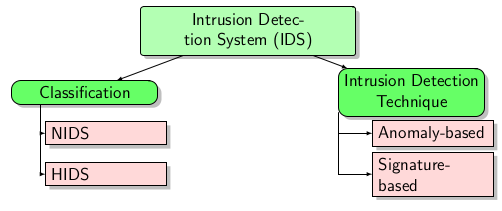
\includegraphics[width=0.8\textwidth]{Figures/IDS}
\decoRule
\caption{Fonctionnement des systèmes de détection d’intrusions}
\label{fig:IDS_Architecture}
\end{figure} 

\subsection{Les approches}
\label{approchesIDS}
Il existe deux approches d’IDS :\\
\begin{itemize}
\item[-]\textbf{Le NIDS} (Network Based IDS) assure la sécurité au niveau réseau. Il va donc écouter tout le trafic du réseau et générer des alertes en cas de comportement anormal.\\
\item[-]\textbf{Le HIDS} (Host Based IDS) réside sur une machine en particulier. Il surveille et analyse le trafic de la machine hôte pour déceler des intrusions ou des attaques (DoS par exemple). \\
\end{itemize}
Ces deux approches peuvent être fusionnées afin d’améliorer la précision de détection d’intrusion ; il en résulte l’approche hybride.

\subsection{Les méthodes de détection d’intrusions} 
Il existe trois méthodes principales de détection d’intrusions:\\
\begin{itemize}
\item[•]\textbf{Détection par scénario} (Misuse Detection) : pour détecter les attaques, elle utilise une grande base de données qui contient les attaques connues et les associe aux caractéristiques des événements qui se produisent lors d’une attaque similaire. Cette technique est aussi appelée la détection basée sur la signature (Signature-Based Detection) ou la détection basée sur la connaissance (Knowledge-Based Detection).\\
\item[•]\textbf{Détection basée sur l’anomalie} (Anomaly-Based Detection) : utilise un profil qui représente les activités qui ne présentent aucune menace d’une éventuelle attaque ou une préparation d’attaque. Les événements sont par la suite comparés à ce profil d’activités.\\
\item[•]\textbf{Analyse de protocole avec état} (SPA) : commence par définir un ensemble de contraintes qui représente le comportement autorisé d’un programme ou un protocole donné. Le système surveille les opérations exécutées par le programme ou le protocole et vérifie s’ils respectent les contraintes définies par le système. 
\end{itemize} 

\subsection{Les méthodes de collection d'informations sur les flux}
Les IDS collectent les informations sur les flux en utilisant une des deux méthodes suivantes:\\
\begin{itemize}
\item[-] \textbf{Première méthode:} collecter les statistiques sur les flux calculés par les switches OpenFlow.\\
\item[-] \textbf{Deuxième méthode:} capturer les paquets avec leur renfilage et extraire les informations contenues dans ces paquets. 
\end{itemize}

\subsubsection{A) Utilisation des statistiques OpenFlow:}
La plupart des solutions de détection d’intrusions dans les SDN utilisent les statistiques calculées par les switches OpenFlow. Dans ce type de solution, l’IDS est implémenté sous forme d’application SDN qui demande périodiquement les statistiques concernant les flux en utilisant le protocole OpenFlow. Les statistiques sont par la suite analysées au niveau de cette application SDN pour détecter l’intrusion. Les méthodes d’analyse sont basées sur des méthodes statistiques ou d’apprentissage automatique.

\subsubsection{B) Utilisation de l’apprentissage automatique:}
Le principe de ce type de solutions est d’utiliser un dataset (un ensemble de données) présentant des caractéristiques extraites de différents flux de paquets pour entrainer un système intelligent capable de prendre en entrée un vecteur de caractéristiques décrivant un flux de paquets et le classifier comme flux d’attaque ou flux bénins. L’efficacité de ce type de solutions est directement liée au choix du dataset, aux caractéristiques utilisées et au modèle d’apprentissage automatique.

\subsection{Évaluation des performances d'un NIDS}
\label{evaluation}
L'efficacité du NIDS est évaluée par plusieurs paramètres. Une matrice de confusion est un tableau qui est souvent utilisé pour calculer les performances d'un NIDS. Elle est décrite dans le tableau suivant.
\begin{table}[h]
	\begin{center}
		\begin{tabular}{  | m{4cm} | m{4cm} | m{4cm} | }
			\multicolumn{3}{c}{Prédiction}\\
			\hline
			Classe réelle  & Anomalie & Légitime\\
			\hline
			Anomalie & Vrai Positif (VP) & Faux Négatif (FN)\\
			\hline
			Légitime & Faux Positif (FP) & Vrai Négatif (VN)\\
			\hline
		\end{tabular}
		\caption{Matrice de confusion}
	\end{center}
	\label{table:NIDS_Evaluation}
\end{table}

\begin{itemize}
	\item[• VP] : Le nombre d’enregistrements anomalies correctement classés.\\
	\item[• VN] : Le nombre d’enregistrements normaux correctement classés.\\
	\item[• FP] : Le nombre d’enregistrements normaux mal classés.\\
	\item[• FN] : Le nombre d’enregistrements anomalies mal classés.\\ 
\end{itemize}

Afin d'évaluer le NIDS, les métriques suivantes sont calculées :\\
\begin{itemize}
	\item[•] \textbf{Exactitude (E)}: Indique le pourcentage de prédictions correctes sur la totalité des prédictions:
	\begin{large}
		\begin{center}
			$ E = \frac{VP + VN}{ VP + VN + FP + FN} \times 100\% $
		\end{center}
	\end{large}
	
	\hfill
	
	\item[•] \textbf{Précision (P)}: Indique combien d’intrusions prédites par un NIDS sont réellement des intrusions. Plus la précision est élevée, plus le taux de fausse alerte est faible:
	\begin{large}
		\begin{center}
			$ P = \frac{VP}{ VP + FP} \times 100\%$
		\end{center}
	\end{large}
	
	\hfill
	
	\item[•] \textbf{Rappel (R)}: Pourcentage des intrusions prédites par rapport à toutes les intrusions présentées:
	\begin{large}
		\begin{center}
			$ R = \frac{VP}{ VP + FN} \times 100\%$
		\end{center}
	\end{large}
	
	\hfill
	
	\item[•] \textbf{F1-Measure (R)}: Une mesure qui combine la précision et le rappel:\\
	\begin{large}
		\begin{center}
			$ R = 2 \times \frac{1}{ \frac{1}{P} + \frac{1}{R}} \times 100\%$
		\end{center}
	\end{large}
	
	\hfill
	
	\item[•] \textbf{Taux de faux Positif (TFP) et Taux de vrai Positif (TVP)}:\\
	\begin{large}
		\begin{center}
			$ TFP = \frac{FP}{ VN + FP} \times 100\%$ , $ TVP = \frac{VP}{ VN + FP} \times 100\%$ 
		\end{center}
	\end{large}
\end{itemize}

\section{Travaux existants}
Récemment, diverses solutions ont été proposées pour régler les problèmes de sécurité au sein des réseaux SDN. Les techniques d’apprentissage automatique sont largement appliquées pour améliorer l’efficacité de détection, y compris les réseaux neurone, les arbres de décision, les SVM (Support Vector Machine) et les réseaux bayésiens. L'intégration d'un système de détection d'intrusions dans l'architecture SDN reste la meilleure solution pour sécuriser l'environnement SDN. Comme mentionné dans la section \ref{approchesIDS}, deux approches existent pour concevoir un IDS : l'une est basée machine (HIDS) et l'autre est basée réseau (NIDS), autrement appelé basé flux. Dans notre travail nous nous focaliserons sur les systèmes de détection basés flux, donc nous allons présenter dans ce qui suit quelques IDS déjà existants afin de pouvoir faire une étude comparative; technique d'apprentissage adoptée, les caractéristiques utilisées, le dataset, résultat de prédiction.\\

\newpage
\subsection{Flow based Intrusion Detection System [\cite{11}]:}
Les auteurs de ce travail ont proposé un système de détection basé flux pour détecter le trafic anormal circulant dans les réseaux SDN. Leur IDS est basé sur l’extraction d’un ensemble de caractéristiques prédéfinies de manière régulière chaque seconde. Cette étape est suivie par l’agrégation des caractéristiques extraites pour pouvoir entraîner le modèle. La figure \ref{fig:NIDS1} illustre l'architecture de cet IDS.
\begin{figure}[h]
\centering
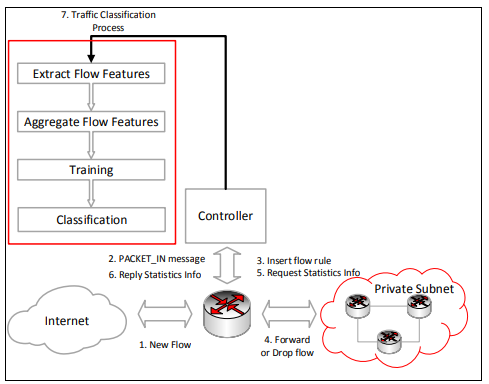
\includegraphics[width=0.6\textwidth]{Figures/NIDS1}
\decoRule
\caption{IDS [\cite{11}]}
\label{fig:NIDS1}
\end{figure}

\subsubsection{A) Extraction et agrégation des caractéristiques:}
Les commutateurs OF envoient souvent des messages \textit{Packet-In} au contrôleur quand aucune correspondance n’est trouvée dans la table de flux du commutateur. Chaque message contient les informations du premier paquet de chaque flux et quand il est reçu au niveau du contrôleur ces informations sont extraites et sauvegardées. En plus, ce qui est bien avec les SDN, ces commutateurs peuvent envoyer des statistiques pour chaque entrée de flux, ce qui permettra la collecte d'informations de flux chaque seconde. 

\subsubsection{B) Entraînement du modèle et la classification:}
Les échantillons extraits de la phase d’agrégation sont utilisés dans un modèle de classification supervisé. Par conséquent, le classifieur formé attribuera des classes à chaque échantillon chaque seconde. Puisque chaque flux peut avoir plus d’une instance au cours de sa durée de vie, son comportement sera classé plusieurs fois. Le classifieur \textit{Bagged-Trees} [\cite{12}] a été utilisé pour construire le modèle.
\newpage
\subsection{Machine based Intrusion Detection System [\cite{13}]:}
Dans ce travail un modèle de réseaux de neurones a été intégré dans le système pour détecter les anomalies dans le trafic. Le système fonctionne comme suit : les commutateurs OF envoient périodiquement les statistiques de flux au contrôleur, ces statistiques vont être récupérées et traitées par le module responsable pour détecter le comportement d’anomalie dans le flux. Pattern recognition (la reconnaissance de motifs) est implémentée dans ce modèle pour classer les entrées dans un ensemble de catégories cibles. L’architecture de cet IDS se compose de trois couches : une couche d’entrée (Input Layer), une couche cachée (Hidden Layer) et une couche de sortie (Output Layer). L’algorithme "\textbf{Backpropagation}" est utilisé pour entraîner le modèle.\\

\begin{table}[h]
\begin{center}
\begin{tabular}{  | m{4cm} | m{5cm} | m{5cm} | }
\hline
IDS & Machine based Intrusion Detection System [\cite{13}] & Flow based Intrusion Detection System [\cite{11}]\\
\hline
Technique d’apprentissage automatique & Neural Network & Bagged Trees\\
\hline
Caractéristiques utilisées & \begin{itemize}
\item[-] Durée
\item[-] Type de protocole
\item[-] Nombre d’octets source-destination
\item[-] Nombre d’octets destination-source
\item[-] Nombre de connections avec le même hôte
\item[-] Nombre de connections vers le même service
\end{itemize} &\begin{itemize}
\item[-] Durée de mesure
\item[-] Nombre de paquets
\item[-] Nombre d’octets
\item[-] Variation dans la durée du flux
\item[-] Variation dans le nombre de paquets
\item[-] Variation dans le nombre d’octets
\end{itemize} \\
\hline
Dataset & NSL-KDD (standardisé) crée en 1999 & Généré avec une émulation de l’environnement SDN (non standardisé) publiée en 2017 \\
\hline 
Type d’attaques dans le dataset  & \begin{itemize}
\item[-] DoS
\item[-] Remote2Local
\item[-] User2Root
\item[-] Probe
\end{itemize} &\begin{itemize}
\item[-] DoS
\item[-] Http brute force
\item[-] SSH brute force
\end{itemize}\\
\hline
\end{tabular}
\caption{Comparaison entre les deux IDS proposés}
\end{center}
\label{table:IDS}
\end{table}

\begin{tabular}{| m{4cm} | m{5cm} | m{5cm} |}
\multicolumn{3}{c}{Résultats expérimentaux}\\
\hline
Taux de vrai Positif & 0.941 & 0.9834\\
\hline
Taux de faux Positif & 0.005 & 0.016\\
\hline
Exactitude & 0.973 & Non mentionnée \\
\hline
\end{tabular}

\subsection{Comparaison de ces deux IDS}
Nous remarquons que les deux solutions donnent des résultats de performances très intéressants. Les auteurs de la solution [\cite{11}] n’ont pas mentionné le taux de faux négatifs qu’est un élément très important dans l’évaluation d’un IDS. L’utilisation d’un dataset non standardisé dans [\cite{11}] est discutable sur le plan de la validité des attaques, les flux générés et le bon déroulement de l’extraction des informations et caractéristiques lors de la création du dataset. La solution [\cite{13}] utilise un ancien dataset(NSL-KDD créé en 1999) qui s’avère dépassé dû aux grands changements dans les réseaux, et l’apparition de nouveaux types d’attaques récentes. Par conséquent, l’IDS peut être inefficace face aux attaques récentes ainsi que dans la reconnaissance des caractéristiques des flux normaux modernes.\\
D’après cette étude nous constatons qu’il est nécessaire de mettre en place une solution de détection des attaques DoS dans les SDN qui prend en considération les critiques susmentionnées. 

\section{Conclusion}
Dans ce chapitre nous avons tout d’abord étudié les problèmes de sécurité dans l’environnement SDN. Nous avons ensuite présenté quelques solutions déjà proposées pour détecter les attaques DoS. Dans le chapitre suivant, nous allons nous familiariser avec la technique d’apprentissage que nous utiliserons pour la conception de nore solution. 

% Chapter 3
\chapter{Data Mining}

\label{Chapter3} 
Pour construire n'importe quel modèle de prédiction, il est nécessaire de choisir une technique d'apprentissage automatique ainsi qu'un Dataset pour traîner le modèle. Dans ce chapitre nous allons parler sur les Dataset, comment choisir et évaluer un Dataset, nous parlerons aussi sur l’apprentissage automatique ainsi que ses deux grandes classes. Cette discipline de traitement de grandes quantité de données et choix de modèles et connue sous le nom de \textit{Data-Mining}.

\section{Data Minig}
\subsection{Définition}
L’exploration de données, connue aussi sous l’expression de fouille de données, forage de données, prospection de données, a pour objet l’extraction d’un savoir ou d’une connaissance à partir de grandes quantités de données, par des méthodes automatiques ou semi-automatiques. Le processus le plus connu du Data-Mining est le KDD (knowledge discovery in database)[\cite{11}], appelé en français extraction de connaissances à partir de données ou processus de découverte de connaissances.

\subsection{Ètapes du processus KDD}
\label{KDD}
Le processus KDD est sur trois étapes comme suit:\\
\begin{itemize}
\item[1-]\textbf{Préparation des données} : Elle comprend la collecte, l'intégration, la transformation, le nettoyage et la réduction des données. Dans notre cas la Collecte d'information est faite en capturant le trafic réseau à l'aide du \textit{port-mirroring} des équipements réseau.\\
\item[2-]\textbf{Recherche des modèles} : Consiste à appliquer l'analyse des données et les algorithmes de découverte qui produisent une énumération de modèles sur les données.\\
\item[3-]\textbf{Évaluation des modèles} : Consiste à estimer l'erreur et la précision sur les modèles extraites.Un modèle est considéré comme une connaissance s'il dépasse un certain pourcentage de précision.
\end{itemize}

\subsection{Dataset}
Pour concevoir notre modèle d'apprentissage on a besoin d'une grande quantité de données qui représente plusieurs flux, malins et bénins, capturés dans un réseau. Le choix du bon Dataset contenant ce type de données est cruciale pour construire notre modèle de prédiction. Dans ce qui suit quelques propriétés à prendre en considération lors du choix d'un Dataset [\cite{12}].\\
\begin{itemize}
\item[•]\textbf{Year of Creation}: Étant donné que le trafic réseau est soumis à de nouveaux scénarios d’attaque apparaissent quotidiennement, l’âge d’un ensemble de données de détection d’intrusion joue un rôle important. Cette propriété décrit l’année dans laquelle le trafic a été capturé.\\
\item[•]\textbf{Normal User Behavior}: Cette propriété indique la disponibilité du comportement normal de l’utilisateur dans un ensemble de données et prend les valeurs \textbf{Oui} ou \textbf{Non}. La valeur \textbf{Oui} indique qu’il y a un comportement normal dans l’ensemble de données. En général, la qualité d’un IDS est principalement déterminée par son taux de détection des attaques et son taux de fausses alarmes. Par conséquent, la présence d’un comportement normal est indispensable pour évaluer un IDS.\\
\item[•]\textbf{Attack Traffic}: Un Dataset pour IDS devrait contenir divers scénarios d’attaque. Cette propriété indique la présence de trafic réseau malicieux dans le Dataset.\\
\item[•]\textbf{Kind of Traffic}: La propriété Type de trafic décrit trois origines possibles du trafic réseau : réel, émulé ou synthétique. Réel signifie que le trafic réseau réel a été capturé dans un environnement réseau en production. Émulé signifie que le trafic réseau réel a été capturé dans un banc d’essai ou un environnement réseau émulé. Synthétique signifie que le trafic réseau a été créé synthétiquement (par exemple, par un générateur de trafic) et non capturé par un dispositif réseau réel.\\
\item[•]\textbf{Balanced}: Pour la phase d'apprentissage les données doivent être équilibrés et respectent  leurs étiquettes de classe. Cette propriété indique si le Dataset est équilibré. Un Dataset déséquilibré devrait être équilibrés selon des méthodes appropriées, avant de passer au algorithme d'apprentissage.\\
\item[•]\textbf{Labeled}: Un Dataset étiqueté est nécessaire pour traîner et tester les modèles d’apprentissage, supervisés et non-supervisés. Cette propriété indique si le Dataset est étiqueté ou non. 
\end{itemize}

\begin{table}[h]
\begin{center}
\begin{tabular}{   m{4cm} | m{10cm}  }
\textbf{Dataset} & \textbf{Attaques}\\
\hline
\rowcolor[rgb]{0.85,0.85,0.85}
CICDoS [\cite{13}]  & Attaques DoS sur la couche d'application (ddossim, Goldeneye, hulk, RUDY, Slowhttptest,Slowloris).\\
\hline
CICIDS 2017 [\cite{14}] & Botnet, DoS, DDoS, infiltration, SSH brute force, Injection SQL.\\
\hline
\rowcolor[rgb]{0.85,0.85,0.85}
CIDDS-001 [\cite{15}] & DoS, port scans, SSH brute force.\\
\hline
DDoS 2016 [\cite{16}] & DDoS(HTTP Flood, ICMP Flood, UDP Flood).\\
\hline 
\rowcolor[rgb]{0.85,0.85,0.85}
CICIDS 2018 [\cite{17}] & DoS, FTP and SSH brute force, Botnet, Infiltaration, DDoS.\\
\hline
CICDDoS 2019 [\cite{18}] & Attaques DDoS Reflectives.\\
\hline
\end{tabular}
\caption{Quelques Datasets disponibles pour les système de détection d'intrusions}
\end{center}
\label{table:Datasets}
\end{table}


\newpage
\section{Apprentissage automatique}
L’apprentissage automatique est un concept de développement, d’analyse et d’implémentation qui permet à une machine d’apprendre d’une manière automatique la résolution de problèmes qui s’avéraient complexe à traiter en utilisant les algorithmes classiques.\\

\noindent L’apprentissage automatique est utilisé pour résoudre plusieurs types de problèmes complexes dont la classification et la régression. Le problème de classification s’agit de classifier des données ou des instances en plusieurs classes selon les caractéristiques de ces derniers. Par exemple, apprendre à reconnaître si un flux est bénin ou malin est un problème de classification binaire ; décider le type d’une attaque parmi plusieurs types d’attaques possibles est un problème de classification multi-classes. Les problèmes de régressions sont des problèmes d’approximation des valeurs continues d’une certaine fonction. Par exemple, apprendre à prédire la température pour un jour donné connaissant les diverses conditions atmosphériques.\\

\noindent Les algorithmes d’apprentissage automatique sont classés sous deux grandes classes. Cette classification est directement liée à l’inclusion ou pas d’étiquettes dans l’ensemble de données.

\subsection{Apprentissage supervisé}
L’apprentissage supervisé est un système qui fournit à la fois les données en entrée et les données attendues en sortie. Les données en entrée et en sortie sont étiquetées en vue de leur classification, afin d'établir une base d'apprentissage pour le traitement ultérieur des données. Les systèmes d'apprentissage automatique supervisé alimentent les algorithmes d'apprentissage avec des quantités connues qui étayeront les futures décisions. Ils sont associés pour la plupart à une intelligence artificielle basée sur la récupération, mais ils peuvent aussi reposer sur un modèle d'apprentissage génératif.\\

\noindent Les données utilisées pour l'apprentissage supervisé sont une série d'exemples comprenant des paires composées de sujets en entrée et de sorties attendues. Les modèles d'apprentissage supervisé présentent certains avantages sur les modèles non supervisés, mais ils ont aussi des limites. Par exemple, ils sont plus susceptibles de prendre des décisions auxquelles les humains peuvent s'identifier parce qu'elles reposent sur des données fournies par les humains. Mais dans le cas d'une méthode basée sur la récupération, les systèmes d'apprentissage supervisé ont des difficultés à traiter les nouvelles informations. Si un système qui connaît deux catégories de flux, le flux d’une attaque SYN-Flooding et le flux bénin par exemple, reçoit un flux d’une attaque UDP-Flooding, il devra le placer dans l'une ou l'autre de ces deux catégories, ce qui sera incorrect. Alors que si le système était génératif, il ne saurait pas forcément reconnaître le type d’attaque UDP-Flooding, mais il serait capable de l'identifier comme appartenant à une autre catégorie. \\

\noindent Parmi les algorithmes d’apprentissage supervisé nous trouvons les machines à vecteur de support (SVM),  AdaBoost (adaptative boosting), k plus proches voisins (k-NN) et les réseaux de neurones convergeant vers un état final précis.

\subsection{Apprentissage non supervisé}
L’apprentissage non supervisé consiste à apprendre à un algorithme d'intelligence artificielle (IA) des informations qui ne sont ni classées, ni étiquetées, et à permettre à cet algorithme de réagir à ces informations sans supervision.\\

\noindent Dans ce mode d'apprentissage, le système d'IA peut regrouper des informations non triées en fonction de leurs similitudes et de leurs différences, même si aucune catégorie n'est indiquée. Les systèmes d'IA capables d'utiliser l'apprentissage non supervisé sont souvent associés à des modèles d'apprentissage génératifs, mais ils peuvent aussi fonctionner avec une approche basée sur la récupération (souvent associée à l'apprentissage supervisé).\\

\noindent Les algorithmes d'apprentissage non supervisé peuvent exécuter des tâches de traitement plus complexes que les systèmes d'apprentissage supervisé, mais ils peuvent aussi être plus imprévisibles. Même si un système d'IA d'apprentissage non supervisé parvient tout seul, par exemple, à faire le tri entre des flux bénins et des flux malins, il peut aussi ajouter des catégories inattendues et non désirées pour y classer des flux inhabituels, créant la confusion au lieu de mettre de l'ordre.
Parmi les algorithmes d’apprentissage non supervisé nous citons K-means clustering (K-moyenne), Dimensionality Reduction (Réduction de la dimensionnalité), Distribution models (Modèles de distribution) et Hierarchical clustering (Classification hiérarchique).\\

\newpage
\paragraph{{\large 3.2.2.1 Clustering}\\\\}
Il s'agit essentiellement d'un type de méthode d'apprentissage non supervisé. Clustering est la tâche de diviser la population ou les points de données en un certain nombre de groupes de sorte que les points de données des mêmes groupes soient plus similaires aux autres points de données du même groupe et différents des points de données des autres groupes. Il s'agit essentiellement d'une collection d'objets sur la base de la similitude et de la dissemblance entre eux.\\

\noindent Le clustering est très important car il détermine le groupement intrinsèque des données non marquées. Il n'y a aucun critère pour un bon clustering. Cela dépend de l'utilisateur, quels sont les critères qu'il peut utiliser pour satisfaire ses besoins. Par exemple, nous pourrions être intéressés à trouver des représentants pour des groupes homogènes (réduction des données), à trouver des groupements utiles et appropriés (“useful” data classes) ou à trouver des objets de données inhabituels (outlier détection). L'algorithme du clustering doit faire quelques hypothèses qui constituent la similitude des points et chaque hypothèse fait des clusters différents et également valides. 

\paragraph{{\large 3.2.2.2 Méthodes de clustering}\\\\}
Parmi les méthodes de Clustering on trouve:\\
\begin{itemize}
\item[-]Méthodes basées sur la densité: ces méthodes considèrent les clusters comme la région dense ayant une certaine similitude et différence des autres régions denses de l'espace. Ces méthodes ont une bonne précision et la capacité de fusionner deux clusters. Exemples : DBSCAN, OPTICS …etc.\\
\item[-]Méthodes basées sur la hiérarchie : les clusters formés dans cette méthode forment une structure de type arbre basé sur la hiérarchie. Les nouveaux clusters sont formés en utilisant ceux précédemment formés.\\
\item[-]Méthodes de partitionnement : ces méthodes partitionnent les objets en k clusters et chaque partition forme un cluster. Cette méthode est utilisée pour optimiser une fonction de similarité de critère objectif comme lorsque la distance est un paramètre majeur. Exemple : K-means, CLARANS …etc.
\end{itemize}

\paragraph{{\large 3.2.2.3 K-Means}\\\\}
K-means est un algorithme non supervisé de clustering non hiérarchique. Il permet d’analyser un jeu de données caractérisées par un ensemble de descripteurs, afin de regrouper les données similaires en groupes (ou clusters). La similarité entre deux données peut être inférée grâce à la “distance” séparant leurs descripteurs ; ainsi deux données très similaires sont deux données dont les descripteurs sont très proches. Cette définition permet de formuler le problème de partitionnement des données comme la recherche de K “données prototypes”, autour desquelles peuvent être regroupées les autres données. Ces données prototypes sont appelées centroïdes ; en pratique l’algorithme associe chaque donnée à son centroïde le plus proche, afin de créer des clusters. D’autre part, les moyennes des descripteurs des données d’un cluster, définissent la position de leur centroïde dans l’espace des descripteurs : ceci est à l’origine du nom de cet algorithme (K-means ou K-moyennes en Français). Après avoir initialisé ses centroïdes en prenant des données au hasard dans le jeu de données, K-means alterne plusieurs fois ces deux étapes pour optimiser les centroïdes et leurs groupes:\\
\begin{itemize}
\item[1-]Regrouper chaque objet autour du centroïde le plus proche.
\item[2-]Replacer chaque centroïde selon la moyenne des descripteurs de son groupe.\\
\end{itemize}

Après quelques itérations, l’algorithme trouve un découpage stable du jeu de données : on dit que l’algorithme a convergé. Comme tout algorithme, K-means présente des avantages et des inconvénients : il est simple, rapide et facile à comprendre ; cependant il ne permet pas de trouver des groupes ayant des formes complexes.

\begin{figure}[h]
\centering
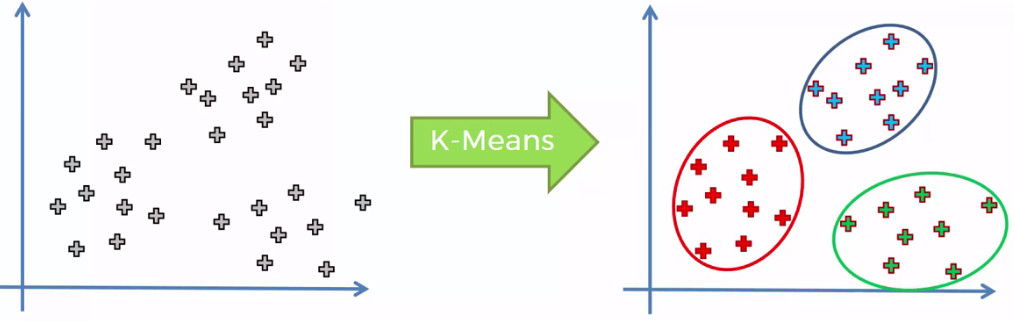
\includegraphics[width=0.8\textwidth]{Figures/K-means}
\decoRule
\caption{K-Means}
\label{fig:K-means}
\end{figure}

\subsection{Conclusion}
Dans ce chapitre nous avons discuté sur le Data-Minig, en commençant par définir c'est quoi cette discipline, pour passer par la suite au dataset en exposant les majeures propriétés à considérer lors du choix d'un dataset. L'apprentissage automatique était la dernière section de ce chapitre, où on a présenté les différentes méthodes et algorithmes d'apprentissage existants. 
% Chapter 4
\chapter{Conception}

\label{Chapter4} 
le Software-Defined Networking a rapidement émergé comme une technologie prometteuse pour les réseaux futurs et a gagné beaucoup d'attention. Cependant, la nature centralisée du SDN rend le système vulnérable aux attaques par déni de service (Dos), une fois le contrôleur compris, tout le réseau cessera de fonctionner. Mais cette centralisation a un avantage, la gestion centralisée des équipements réseau, elle permet d'avoir une vue globale des flux de trafic, ce qui offre un meilleur système de défense contre les attaques DoS.\\

Comme mentionné dans la section \ref{rDoS}, nous nous intéressons dans notre travail à une attaque DOS spécifique, connue sous le nom de \textbf{Reflective-DoS} (RDos). Cette attaque est un peu spéciale et diffère carrément des autres types d'attaques Dos dans le principe de fonctionnement et les dommages causés. nous parlerons plus sur cette attaque dans la section suivante. \\

Nous proposons dans ce chapitre une modélisation de notre solution. Nous commençons par présenter son architecture générale et les différents modules qui le composent. Dans la suite de ce chapitre, nous nous concentrons sur la conception de ces modules et le développement du système en appliquant les notions que nous avons apprises sur les réseaux SDN, les IDS et l’apprentissage automatique.

\section{Problématique}
Mars 2018, un nouveau record a été marqué avec 1.7 Tbps de trafic généré par une attaque DoS réflective. La compagnie \textbf{Arbor Networks} a affirmé que son système d'analyse de trafic, ATLAS, a enregistré 1.7 Tbps d'une attaque reflective contre un site web d'un client[\cite{22}].\\

RDoS n’attaque pas directement la cible mais envoie plutôt plusieurs requêtes vers un service tiers exploitable (c. -à-d. le réflecteur, généralement c'est un serveur) avec une adresse IP d’expéditeur usurpée, ce qui rend l'attaquant anonymat. Les réponses du serveur tiers sont ensuite envoyées à la cible d’attaque réelle et causer une surcharge. Les protocoles avec des messages de réponse qui sont beaucoup plus grands que les messages de demande sont particulièrement bien adapté à ces attaques en raison des effets d’amplification. La nature de ces attaques nécessite des services qui fonctionnent sans connexion établie entre le client et le serveur. Une étude récente[\cite{23}] a trouvé que $ 99.72\% $ des attauqes RDoS utilisent des protocols basé UDP, comme DNS, NTP, ..etc. Les messages reçus dans une attaque RDoS sont difficiles à différencier du trafic bénin, car ils sont conformes aux spécifications du protocole. Les réflecteurs gèrent correctement toutes les demandes comme légitimes, mais l’absence de réponse est une caractéristique des attaques réflectives qui ne peut être masquée.

\begin{figure}[h]
\centering
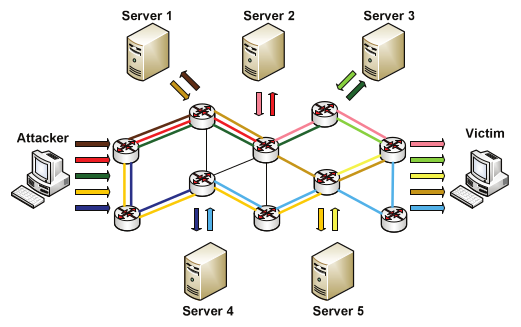
\includegraphics[width=0.75\textwidth]{Figures/rDoS}
\decoRule
\caption{Principe de déni de service réflectif}
\label{fig:rDoS}
\end{figure} 

À ce niveau, nous pouvons clairement voir que l'impact de ce type d'attaque est en double; en premier lieu, la consommation de la bande passante des liens réseau à cause du nombre excessif des messages requêtes et réponses échangés. En deuxième lieu, la surcharge des serveurs tiers avec des messages requêtes, qui vont les traiter évidemment, car pour eux ils paraissent des requêtes légitimes. 

\section{Motivation du travail}
Un article[\cite{24}] sur les travaux connexes a montré que la défense contre les attaques RDoS peut être divisée en 3 principales tâches : (1) surveillance (\textit{monitoring}) et la collecte de données du trafic réseau, (2) l’interprétation de ces données et la détection d’une attaque en cours, et (3) la mitigation de l’attaque. Selon leurs tâches principales, les solutions existantes varient considérablement dans leurs hypothèses et leurs exigences.\\
Dans la littérature on trouve que la surveillance du trafic, qui représente la première phase du processus de détection, se fait sur ces trois couches:\\
\begin{itemize}
\item[•] La couche réseau.
\item[•] La couche de transport.
\item[•] La couche d'application.\\
\end{itemize}
\newpage
Par exemple \textit{PacketScore}, par Kim et al [\cite{25}], utilise les statistiques de paquets collectés pour comparer chaque paquet reçu au trafic bénin et d’attaque pour ensuite lui attribuer une note. Les paquets qui sont similaires au trafic d’attaque sont éliminés. Cette approche nécessite une surveillance active de la couche réseau. Plusieurs autres travaux [\cite{26}, \cite{27}] s'intéressent à la couche de transport pour la détection des anomalies en analysant les paquets de transport, ICMP, TCP et UDP.\\

Pour cette fin, nous proposons une solution, basée sur une approche de clustering, pour la détection des ttaques Dos réflectives dans un réseau SDN. Cette solution prend en charge aussi les attaques DoS du type UDP-Flooding (voir section \ref{rDoS}). La mitigation de l'attaque ne fait pas par partie de notre travail, nous ferons juste la détection. La première tâche, surveillance te collecte de données, va être lancée sur la couche de transport, où on surveillera spécialement le protocole de transport UDP, vu qu'il est le plus utilisé dans les attaques RDoS. Pour la deuxième phase, qui est la détection, nous utiliserons notre modèle d'apprentissage pour analyser les données collectées dans la phase précédente et décider si c'est une attaque ou non.

\section{Présentation de la Solution}
Les caractéristiques inhérentes des attaques de RDoS représentent un défi pour leur détection. Une surveillance et analyse continues du trafic réseau sont nécessaires pour la détection des flux malins. La solution qu'on propose, pour ce fait, est un système de détection, appelé \textbf{F-DoS}, qui sera déployée dans le réseau cible pour assurer la surveillance du trafic au but de détecter les attaques DoS (RDoS et UDP-Flooding).\\

Ces deux fonctions de surveillance et de détection sont assuré par deux modules intégrés dans notre système. Le premier est le module d'extraction d'informations, qu'on référencera par l'acronyme \textbf{MEI}. Une copie de chaque flux circulant dans le réseau est envoyée à ce module afin d'extraire ses caractéristiques. Les caractéristiques extraites sont ensuite envoyées au deuxième module de notre système, appelé \textbf{F-Clustering}, qui est un modèle intelligent, sa fonction est de grouper les flux en clusters, cluster des flux normaux et cluster des flux malins.\\

L'architecture et le principe de fonctionnement de notre système sont illustrés dans la figure suivante: \\

\begin{figure}[h]
\centering
\begin{minipage}[b]{.5\textwidth}
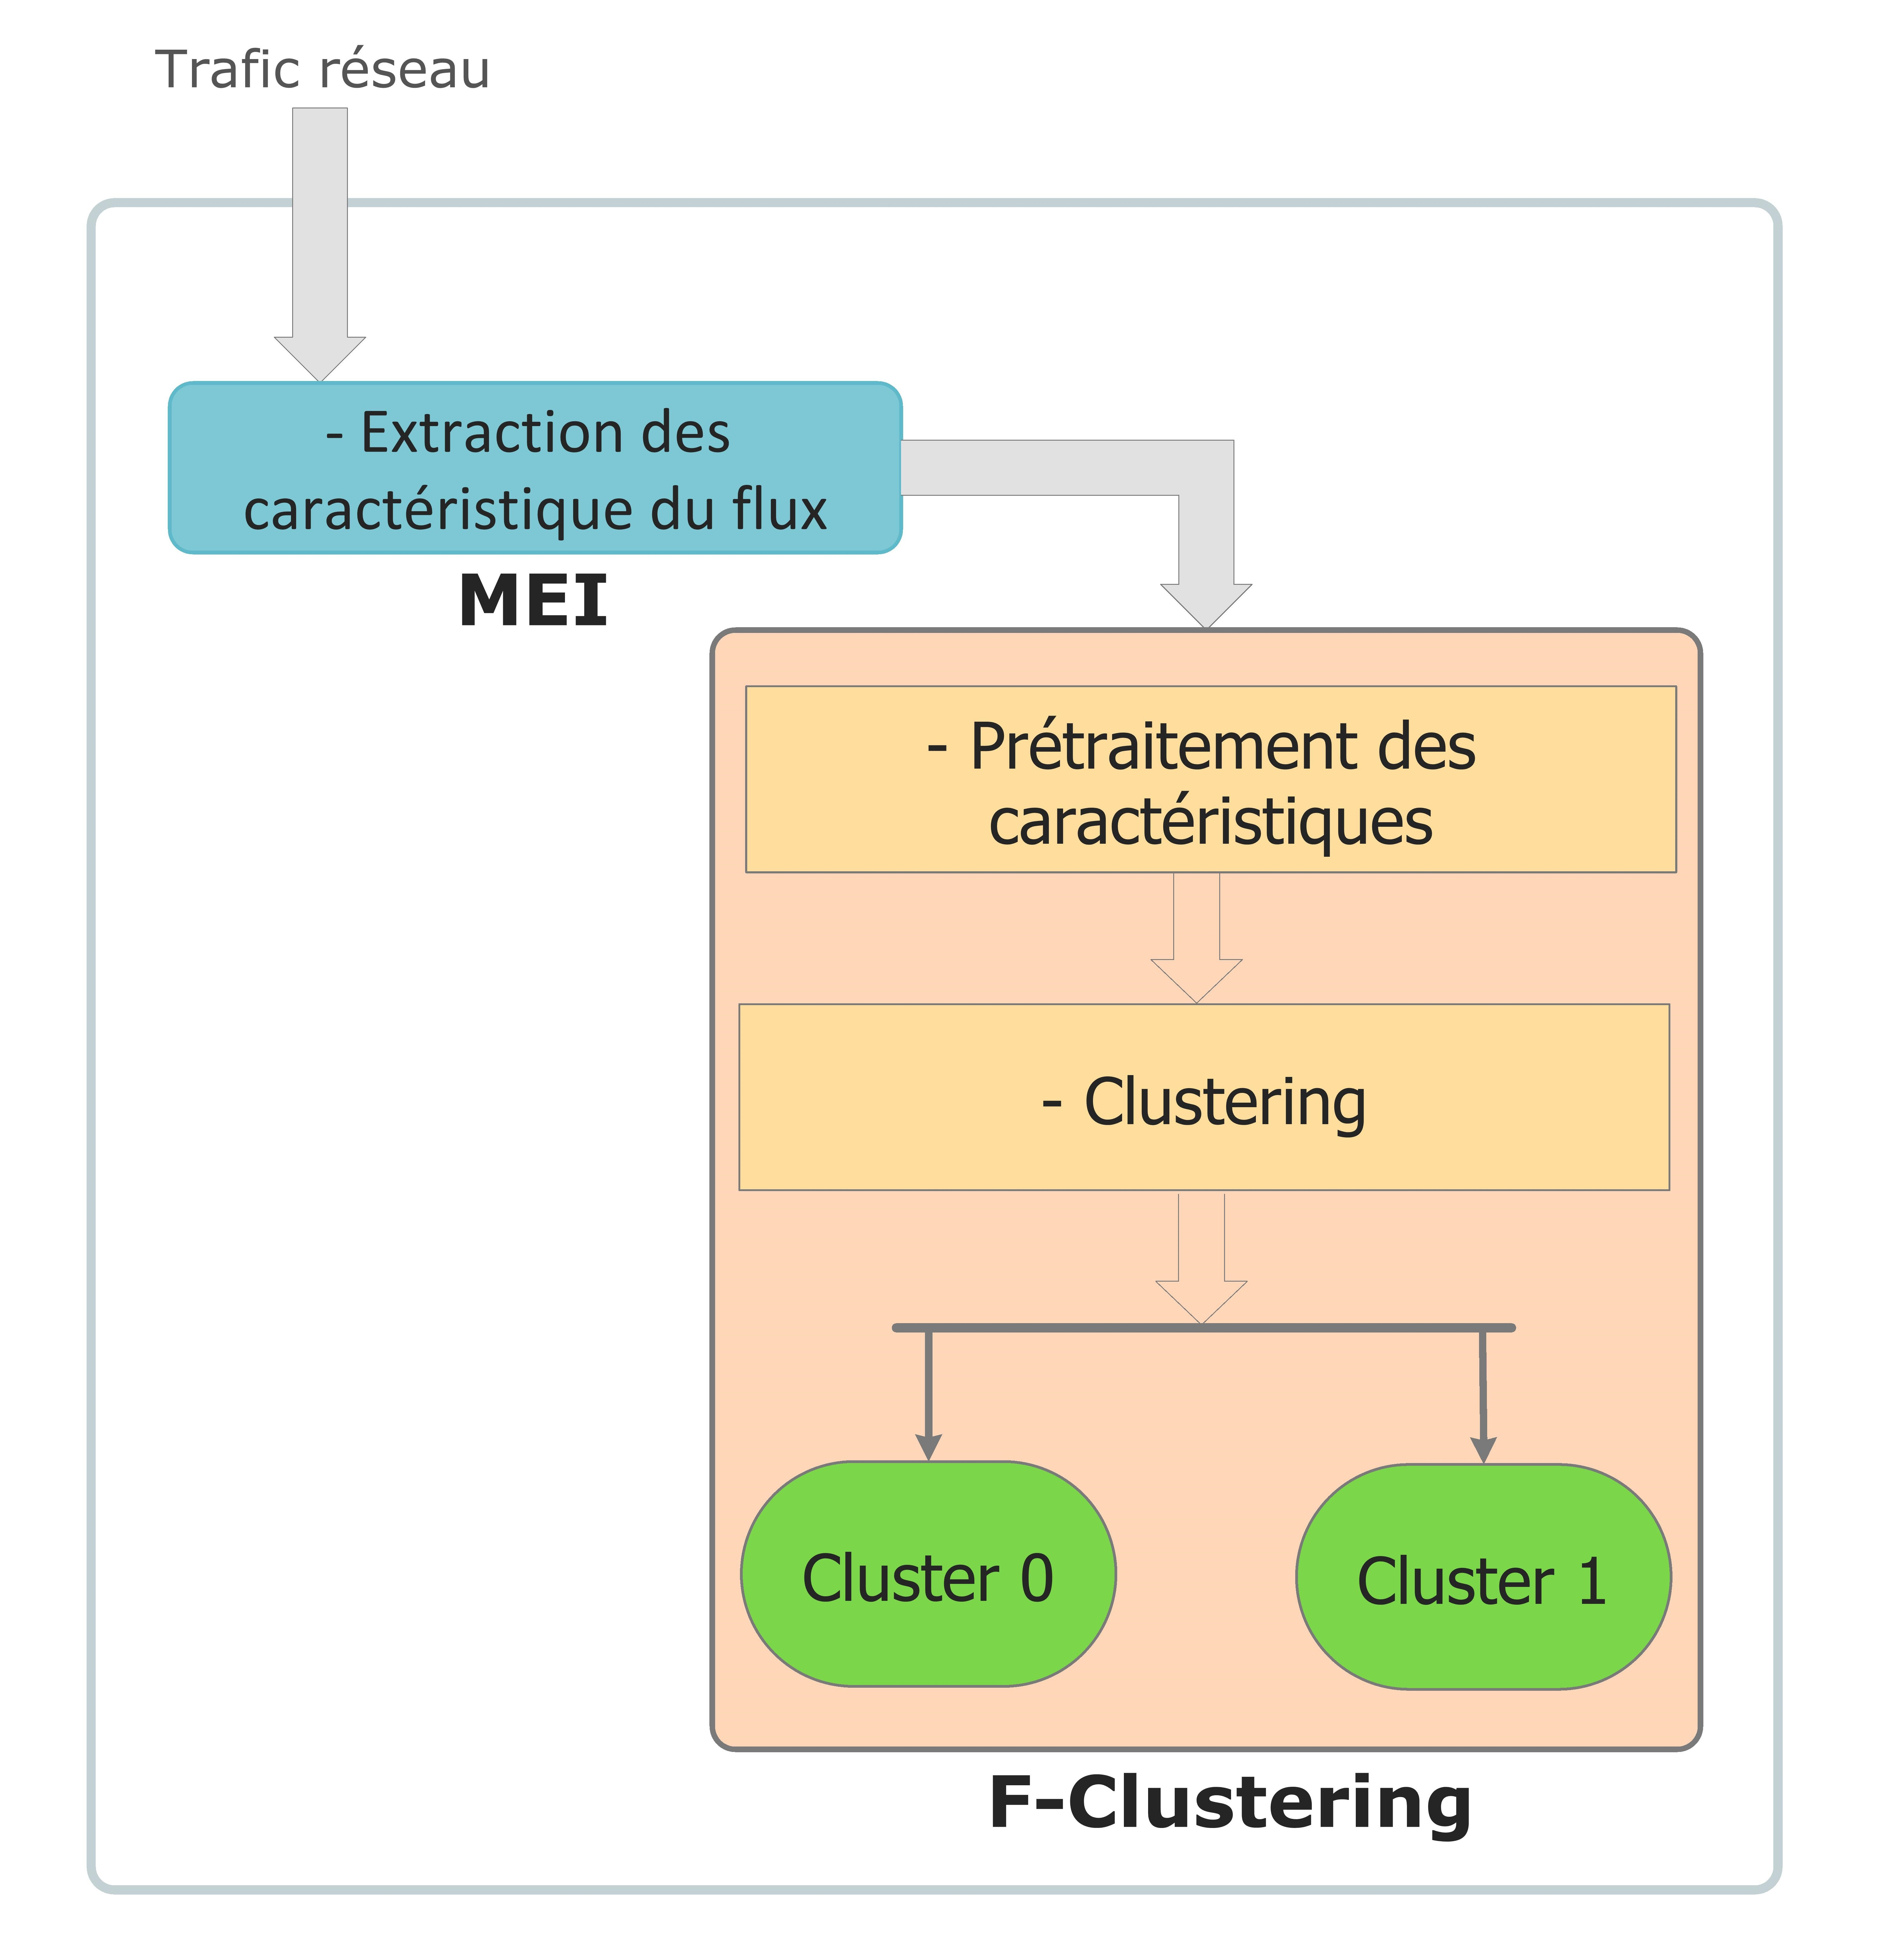
\includegraphics[width=\textwidth]{Figures/F-DoS}
\label{fig:rDoS}
\end{minipage}
\begin{minipage}[b]{.45\textwidth}
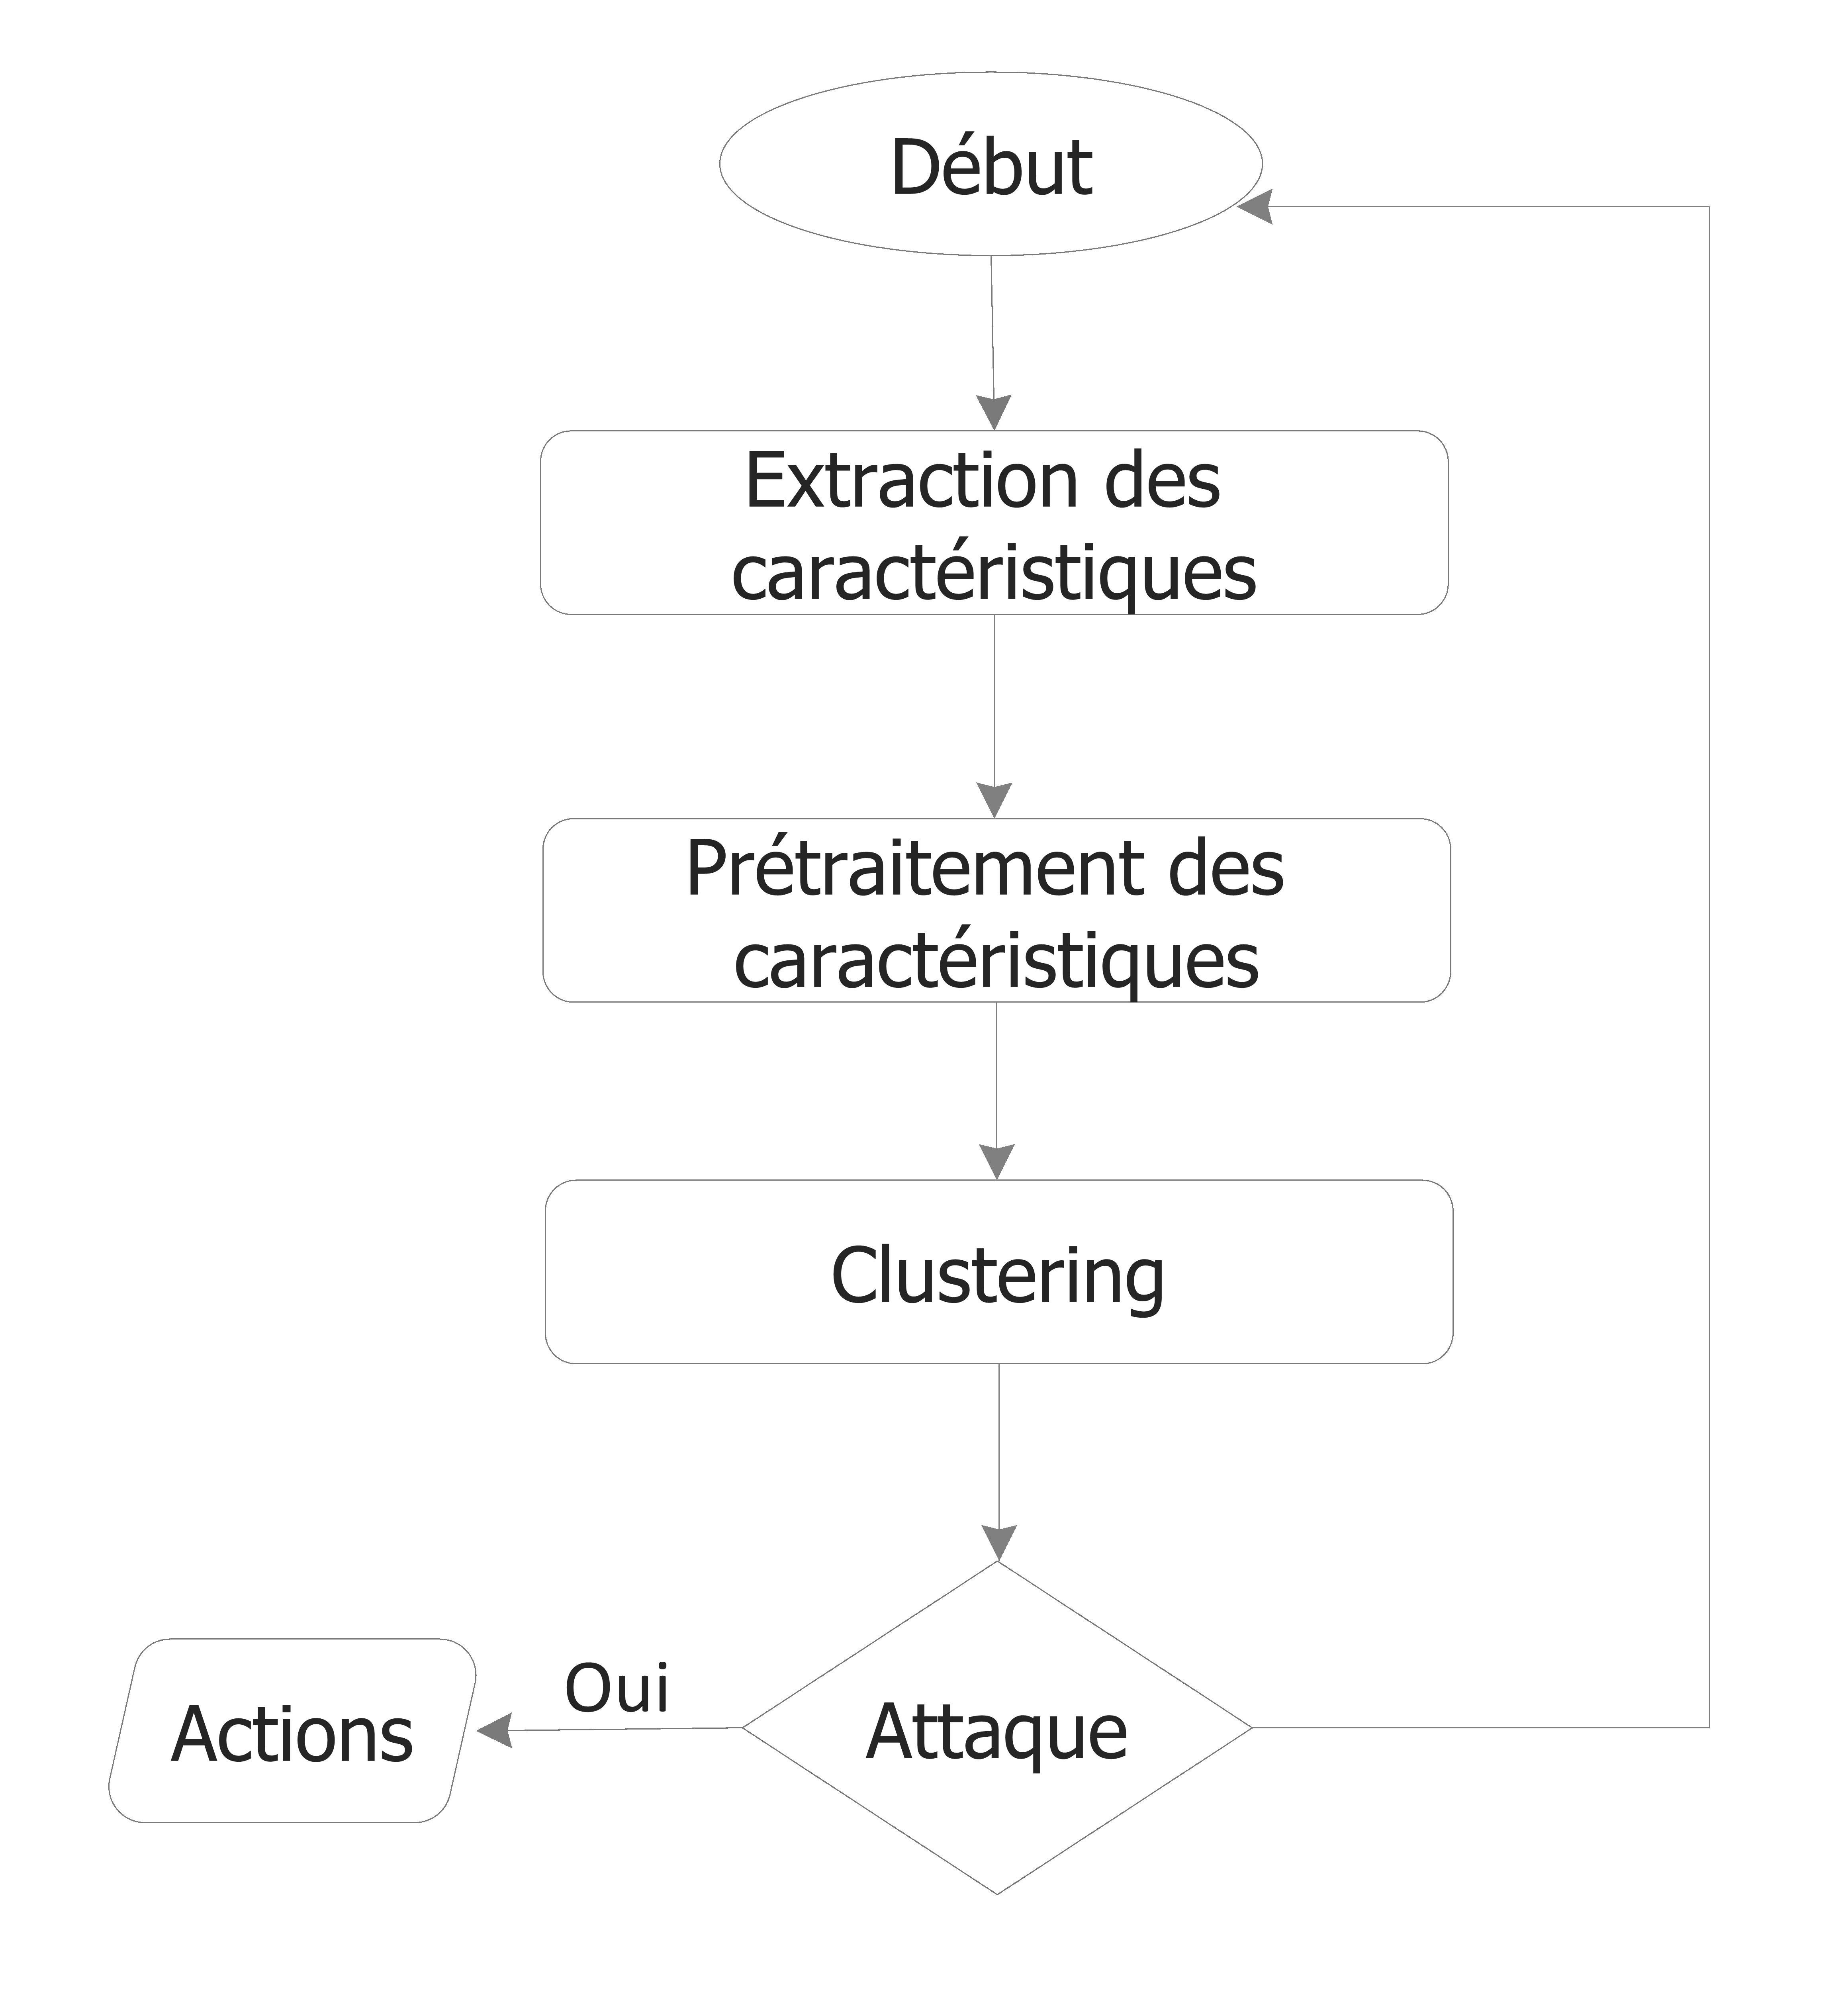
\includegraphics[width=\textwidth]{Figures/Diagramme}
\label{fig:rDoS}
\end{minipage}
\decoRule
\caption{Architecture et fonctionnemnt de F-DoS}
\end{figure}

\newpage
\subsection{Module MEI}
Le rôle principal de ce module est l'extraction des informations des flux de données. Mais pour ce faire, ce module doit assurer trois fonctions: l'écoute, l'analyse et l'extraction. Ce module à un port dédié à l'écoute, qui est toujours active pour recevoir une copie de chaque paquet à l'aide de la technique de mise en miroir \textit{Port Miroring}. L'ensemble des paquets capturés est envoyé par la suite à l'analyseur. L'analyse des paquets n'est pas une fonction simple, elle doit être effectuée soigneusement, si on analyse mal les paquets nous risquons de fausser le résultat de détection. Cette fonction est compliquée a raison que, l'analyseur reçoit tous les paquets qui circulent dans le réseau, et nous avons dit précédemment que nous nous intéressons aux informations des flux de données, un flux est un ensemble de paquets qui partage le même \textit{Paquet Header}(c-a-d même adresse source, adresse destination, port, ... etc). Donc l'analyseur doit calculer les flux en regroupant les paquets communs, identifier les flux de données susceptibles et éliminer tout autre flux no intéressant, comme le flux des messages de contrôle, le flux des messages de sollicitation,...etc. Les flux de données formés vont ainsi être passés à la dernière fonction de ce module pour extraction de caractéristiques de chaque flux.

\newpage
\subsection{Module F-Clustering}
L'objet de notre travail est de proposer une approche de Clustering pour la détection des attaques Dos. Nous nous sommes penchés vers le K-Means, nous l'avons amélioré et adapté à notre utilisation pour construire notre modèle intelligent qui est le coeur de ce module. Ce module prend en entrée le vecteur de caractéristiques construit par le module MEI, et d'après ses préconnaissances, et attribue le flux reçu a un des clusters préexistants. Si le flux est groupé dans le cluster des flux malin on dit qu'une attaque DoS (RDoS ou UDP-Flooding), nous pouvons ainsi lancer une alerte et c'est à l'administrateur réseau de prendre ses dipositions.

\section{Conception du module MEI}
Pour concevoir ce module, nous étions dans l’obligation de choisir un outil d’analyse et de calcul des caractéristiques des flux. Parmi les différents analyseurs existants, nous avons choisi ARGUS[\cite{31}] pour plusieurs raisons:\\
\begin{itemize}
\item[-] Son architecture client/serveur, est simple et personnalisable.
\item[-] Assure les trois fonctions de notre module MEI.
\item[-] Fonctionne en temps réel ce qui permet, par la suite, une détection d'attaques en temps réel.\\
\end{itemize} 
Pour mettre en oeuvre ce module nous avons procédé comme suit:\\
\begin{itemize}
\item[1-] Premièrement, une copie du trafic réseau est redirigée vers ce module à l'aide du \textit{Port-Miroring} activé au niveau des \textit{switches}.\\
\item[2-] Un filtrage est appliqué pour supprimer tout paquet non intéressant pou ce travail.\\
\item[3-] Nous avons lancé le serveur ARGUS pour capturer les flux.\\
\item[4-] Nous avons lancé l’outil ARGUS-client, qui nous permet de sélectionner les caractéristiques et les informations des flux à extraire.\\
\item[5-] Nous traitons par la suite les informations collectées et nous les envoyons au module \textbf{F-Clustering}.\\
\end{itemize}

L'architecture interne du module MEI est illustrée dans la figure \ref{fig:MEI}
\begin{figure}[h]
\centering
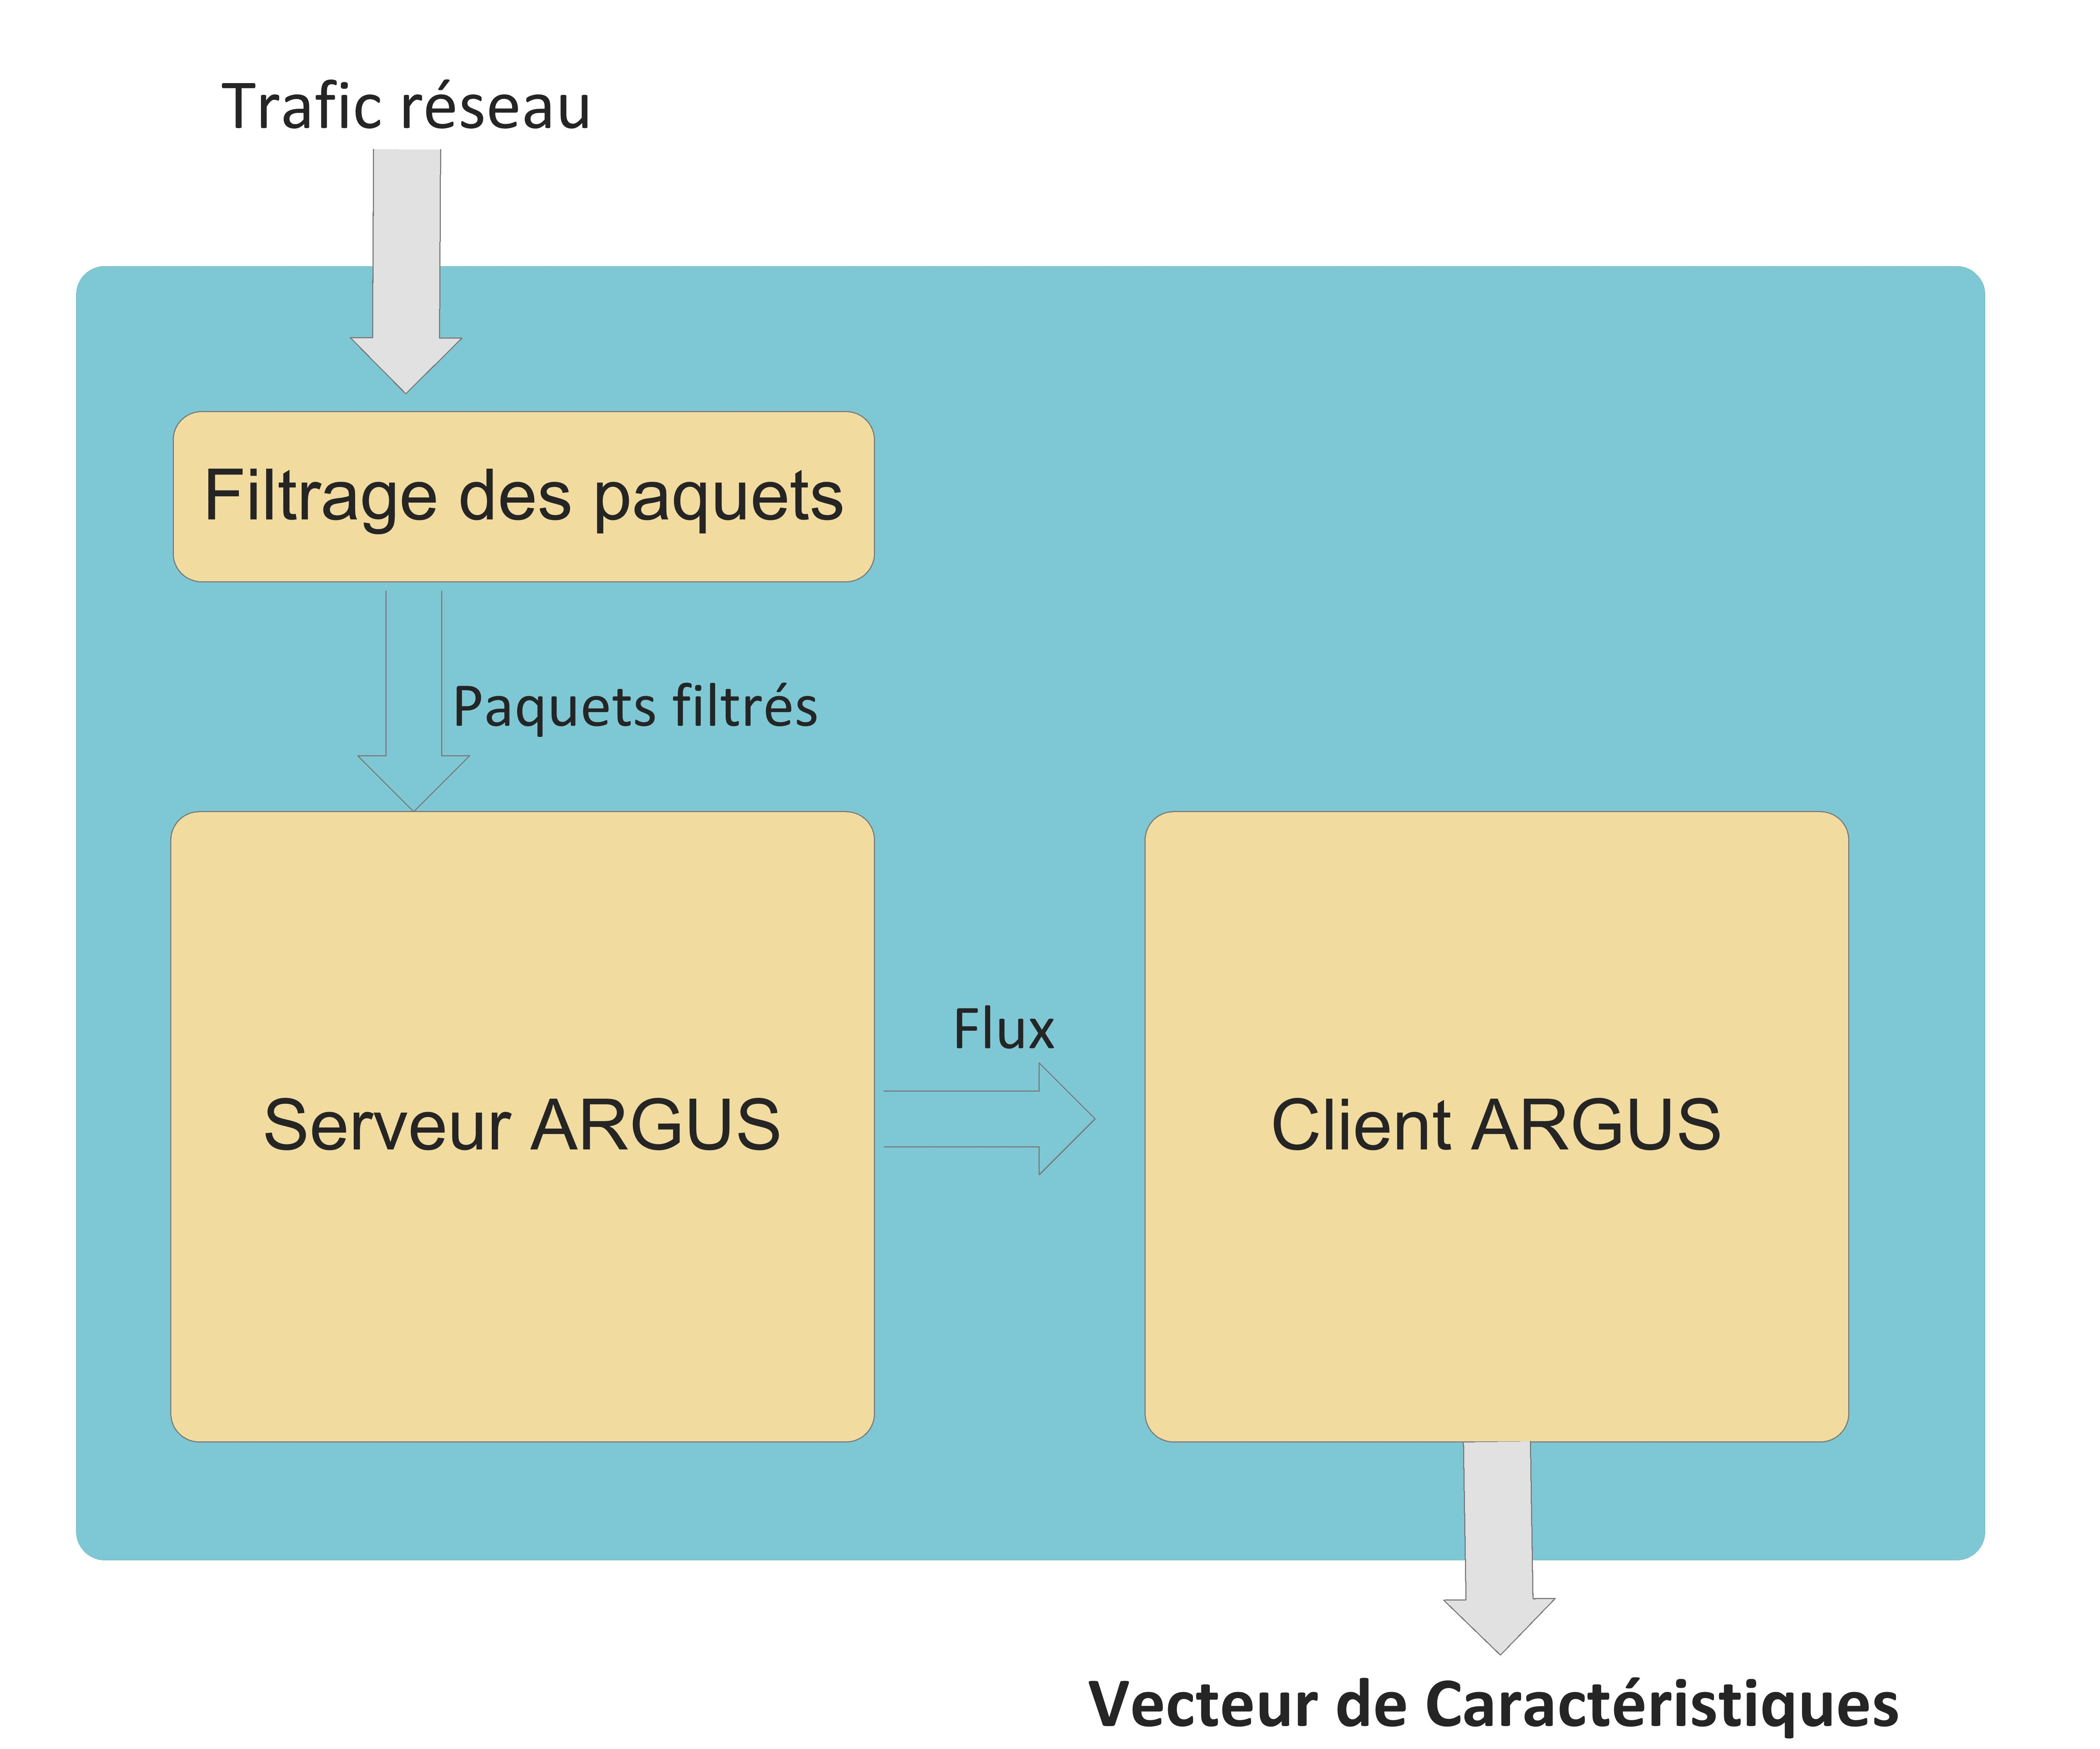
\includegraphics[width=0.6\textwidth]{Figures/MEI}
\decoRule
\caption{Architecture du module MEI}
\label{fig:MEI}
\end{figure} 

\newpage
\section{Conception du module F-Clustering}
\label{F-Clustering}
Pour concevoir ce module nous avons suivi les étapes du processus KDD décrites dans la section \ref{KDD}:\\
\begin{itemize}
\item[-] Préparation des données: premières étapes du processus, où nous parlerons de notre source donnée et les différentes opérations effectuées sur ces données pour les préparer à la deuxième phase du processus. \\
\item[-] Recherche du modèle: le modèle adopté est un modèle d'apprentissage non supervisé, utilisant une approche de Clustering, qui va être trainé sur les données collectées dans la phase précédente.\\
\item[-] Évaluation du modèle: nous ferons l'évaluation du modèle dans le chapitre \ref{Chapter5}.
\end{itemize}

\subsection{Préparation des données}
\subsubsection{A) Choix du dataset }
Comme source de données, nous avons exploité le dataset \textbf{ CICDDoS 2019}[\cite{21}]. CICDDoS2019 contient des flux bénins et des attaques Ddos les plus courantes, qui ressemblent aux vraies données du monde réel. Ce dataset contient différentes attaques DoS modernes réflectives telles que Portmap, Netbios, LDAP, UDP, TFTP, NTP. La période de capture a commencé le 12 janvier à 10 h 30 et s’est terminée à 17 h 15. Des attaques ont par la suite été exécutées au cours de cette période.
\newpage
CICDDoS2019 est formé de plusieurs fichiers, chacun propre à une attaque. Vu la taille énorme de ces fichiers, et pour raison de simplifier le travail et pouvoir simuler l'architecture générale de notre réseau, nous nous sommes mis d’accord sur le choix d'un seul fichier pour travailler sur. Le fichier que nous avons choisi est propre à l'attaque TFTP, qui est lui-même un dataset contenant 20 millions de lignes et 88 colonnes (aussi référées par caractéristiques ou attributs).

\begin{longtable}{ | m{5cm} | m{11cm} | }
\hline
\textbf{Attribut} & \textbf{Déscription}\\
\hline
Source IP/Port & Adresse IP/port source\\
\hline
Destination IP/Port & Adresse IP/port destination\\
\hline
Protocol & Protocole \\
\hline
Flow Duration &  La durée du flux\\
\hline
Total Fwd/Backward Packets & Nombre de paquets transmis/reçus \\
\hline
Total Length of Fwd/Bwd Packets & Taille totale des paquets envoyés/reçus \\
\hline
Fwd/Bwd Packets Length Max/Min/Mean/Std &  Taille maximale/minimale/moyenne/standard des paquets envoyés/reçus\\ 
\hline
Flow Packets/s \& Flow Bytes/s & Nombre de packets/octects transmis par seconde\\
\hline
Flow IAT Mean/Std/Max/Min & Temps de déviation moyen/standard/maximum/ minimum entre deux flux\\
\hline
Fwd/Bwd IAT Tot/Mean/ Std/Max/Min & Temps de déviation total/moyen/standard/maximum/ minimum entre deux paquets envoyés/reçus\\
\hline
Fwd/Bwd PSH/URG & Nombre de fois l'indice PSH/URG a été envoyé/reçu\\
\hline
Fwd/Bwd Header length & Nombre d'octects contenus dans l'ne tête du paquet envoyé/reçu\\
\hline
Fwd/Bwd packets/s & Nombre de paquets envoyés/reçus par seconde\\
\hline
Packet Length Max/Min/Mean/Std & Taille maximale/minimale/moyenne/standard d'un paquet\\
\hline
Packet Length Variance & Variance de la taille d'un paquet\\
\hline
FIN/SYN/RST/ PSH/ACK/URG/ CWE/ECE Flag Count & Nombre de paquet contenat FIN/SYN/RST/PSH/ACK/ URG/CWE/ECE\\
\hline
Down/Up ratio & Ratio de téléchargement/chargement\\
\hline 
Average Packet Size & Taille moyenne d'un paquet\\
\hline
Fwd/Bwd Seg Size/Byts/Bulk Rate Avg & \\
\hline
Subflow Fwd/Bwd Packets/Byts/b/Blk Rate Avg & \\
\hline
Init\_Win\_Bytes\_Forward & \\
\hline
Init\_Win\_Bytes\_Backward & \\
\hline
act\_data\_pkt\_fwd & Nombre de paquets avec au moins 1 octet de données TCP envoyées\\
\hline
min\_seg\_size\_forward & Taille minimale observée d'un segement envoyé\\
\hline
Active Mean/Std/Max/Min & Temps moyen/standard/maximal/minimal durant lequel un flux était actif avant de devenir inactif\\
\hline 
Idle Mean/Std/Max/Min & Temps moyen/standard/maximal/minimal durant lequel un flux était inactif avant de devenir actif\\
\hline
SimilarHTTP & \\
\hline
Inbound & \\
\hline
Label & Étiquette\\
\hline
\caption{Attributs du dataset TFTP}
\label{table:attributs}
\end{longtable}

\subsubsection{B) Prétraitement des données }
Le dataset TFTP n'est pas propre, il contient des données avec des ordres de grandeur différents, des valeurs erronées, des duplicats, il n'est pas balancé et contient des attributs que nous n'avons pas besoin dans notre travail. Un prétraitement est nécessaire pour préparer le dataset en vue de l'utiliser dans l'étape de création du modèle d'apprentissage. Ce processus de prétraitement est sur trois étapes; la première est le nettoyage du dataset, connue dans la littérature sous le nom de \textbf{Data Laundry}. Deuxième étape, sélection des attributs. Troisième étape, mise à l'échelle et balancement du dataset.

\subsubsection{B-1) Data Laundry}
Cette étape consiste à nettoyer le dataset:\\
\begin{itemize}
\item[-] Les lignes contenants des valeurs \textit{"Infinit"} ou \textit{"NaN"} seront supprimées.
\item[-] Suppression des duplicates.
\item[-] Les données vont être formatées en un \textit{datatype} standard.
\end{itemize}

\subsubsection{B-2) Sélection des attributs}
\label{attributs}
La qualité des données de l’ensemble d’apprentissages et des attributs qui les caractérisent forment le succès de la technique de clustering utilisée. La présence de variables redondantes, bruitées et peu corrélées avec le cluster d’un exemple rend le processus d’apprentissage plus difficile.\\

\noindent La détection d’intrusion est le genre d’application pour laquelle la sélection d’attributs peut être bénéfique car elle permet tout au moins d’aboutir aux mêmes performances de reconnaissance à partir d’un nombre de caractéristique moindres.\\

\noindent Nous avons choisi les attributs en analysant les propriétés intrinsèques des données, nous avons éliminé la plupart des attributs de base telles que  les hôtes source et destination, les ports, les flags, ...etc. Nous avons éliminé aussi les attributs de contenu qui sont construit à partir de la charge utile (data) des paquets de trafic tels que le nombre d’échec de connexion.  Car, ce sont des valeurs statiques et n’ont aucun impact sur la détection des attaques.\\

\noindent Le choix final des attributs était: le protocole pour filtrer le trafic et étudier le cas du protocole UDP uniquement, la durée du flux, la taille et le nombre de paquets envoyées et reçus, ainsi que les débits de transfert. Le tableau suivant décrit chacun de ces attributs.
\begin{table}[h]
\begin{center}
\begin{tabular}{ | m{4cm} | m{10cm} | }
\hline
\rowcolor[rgb]{0.85,0.85,0.85}
\textbf{Attribut} & \textbf{Déscription}\\
\hline
Protocol & Protocol de transport\\
\hline
Flow Duration & Durée du flux\\
\hline
Total Fwd Packets & Nombre de paquets envoyées \\
\hline
Total Backward Packets &  Nombre de paquets reçus \\
\hline
Total Length of Fwd Packets & Taille totale des paquets envoyées \\
\hline
Total Length of Bwd Packets & Taille totale des paquets reçus \\
\hline
Flow Bytes/s &  Nombre de Byte par seconde\\ 
\hline
Flow Packets/s &  Nombre de paquets par seconde\\
\hline
Fwd Packets/s & Nombre de paquets envoyées par seconde \\
\hline
Bwd Packets/s & Nombre de paquets reçus par seconde \\
\hline
\end{tabular}
\caption{Déscription des attributs}
\label{table:attributs}
\end{center}
\end{table}

\subsubsection{B-3) Mise à l'échelle et balancement}
La mise à l'échelle consiste à diminuer la grande différence entre les valeurs d'une même caractéristique C. Nous avons utilisé la technique Min-Max Scaler sur ce dataset, qui pour chaque valeur X applique l'opération suivante:
\begin{center}
{\large $ X_{scaled} = \frac{X - X_{min}}{X_{max} - X_{min}} $}
\end{center}
Où :\\
\indent X : valeur à mettre à l'échelle de la caractéristique C.\\
\indent $X_{min}$ : plus petite valeur observée de la caractéristique C.\\
\indent $X_{max}$ : plus grande valeur observée de la caractéristique C.\\

Le dataset TFTP n'est pas balancé, il contient beaucoup plus de flux attaqué que de flux bénin. Si nous l'utilisons sans le balancer, notre modèle va toujours pencher vers le cluster des attaques. L'idée du balancement est de générer de nouveaux échantillons de la classe minoritaire à l'aide de fonctions mathématiques existantes.

\subsection{Recherche du modèle}
Deuxième étape du processus KDD. Nous avons opté pour un modèle de Clustering, où a fait l'implémentation de l'algorithme K-Means avec des modifications pour l'adapter à notre utilisation. Le modèle prend en entrée le dataset construit dans l'étape de prétraitement, applique l'algorithme de clustering pour construire les deux clusters, attaque et bénin. En sortie, nous aurons aura un objet, qui groupe un flux donné dans un des clusters existants. Cet objet n'est rien d'autre que le module \textbf{F-Clustering} de notre système.
\begin{figure}[h]
\centering
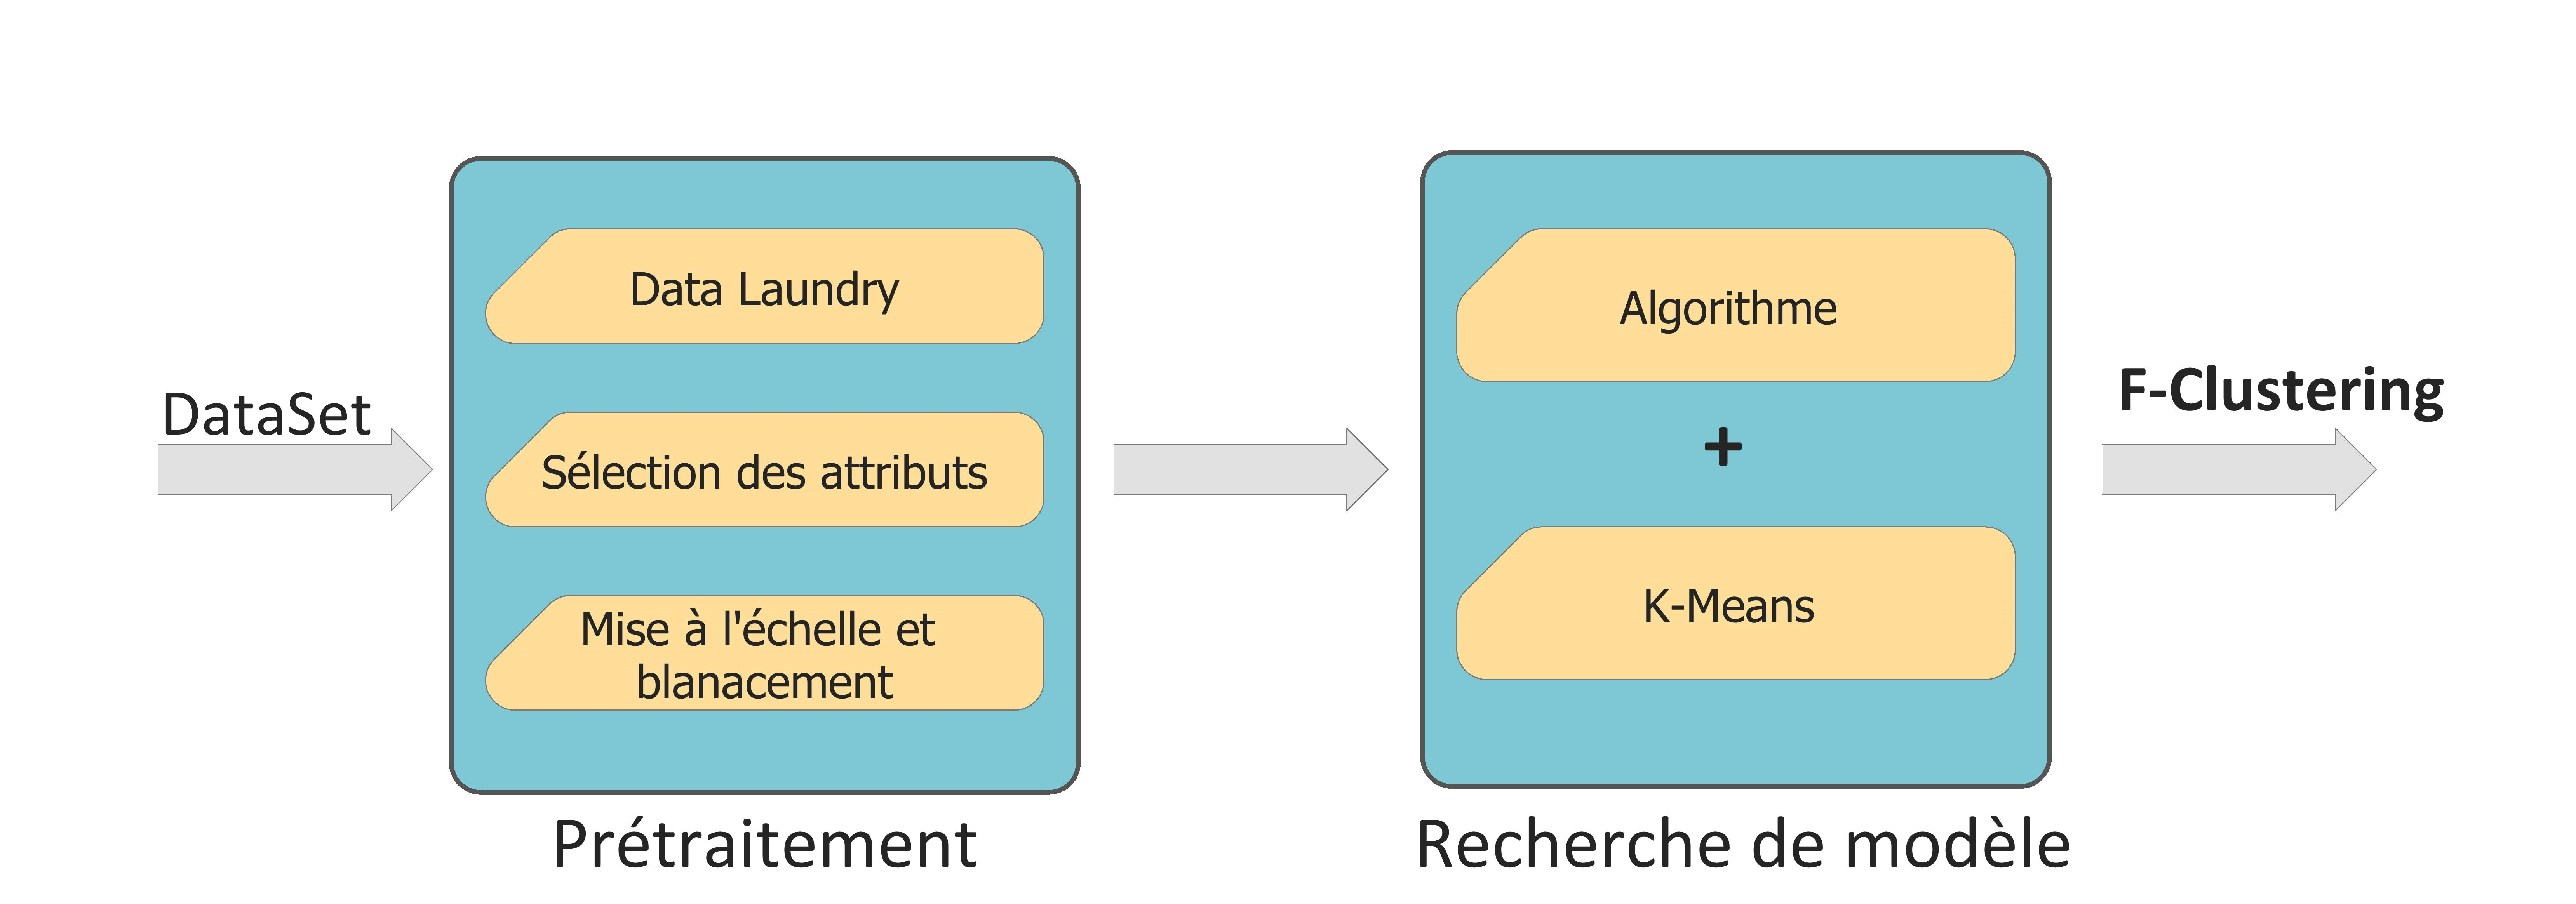
\includegraphics[width=\textwidth]{Figures/Diagramme2}
\decoRule
\caption{Étapes de conception de F-Clustering}
\label{fig:F-Clustering_Diagramme}
\end{figure} 

\section{Module d'archivage}
Nous avons pensé à rajouter, comme fonctionnalité additionnelle à notre système, un module d’archivages qui sauvegarde des logs datés et classés par ordres chronologiques sur les caractéristiques et les informations collectées sur les flux de données.  Une étiquette, qui porte la valeur \textit{"ATTACK"} ou \textit{"BENIGN"}, sera ajoutée à chaque flux, par le modèle de Clustering, pour l'identifier. 57 caractéristiques seront calculées et sauvegardées dans ce module, par exemple : la durée du flux, les adresses source et destination, Timestamp (heure de capture), protocole, ports source et destination, et bien d'autres. Ce module peut servir à plusieurs besoins, par exemple l'analyse périodique du système, il peut servir comme un source de données (dataset) pour d'autres projets qui nécessitent des données fiables et capturées dans un réseau réel. 

\section{Conclusion}
Ce chapitre a porté entièrement sur la conception de notre solution, nous avons commencé par définir la problématique des attaques de déni de service réflectives et décrire la motivation de notre travail. Notre contribution dans ce domaine était un système de détection d'attaques DoS, nous avons vu son architecture générale et détaillé le rôle de chacun des modules qui le composent. Nous avons décrit son fonctionnement et présenté les différentes étapes de conception.\\

\noindent Dans le prochain chapitre, nous allons entamer la partie d'implémentation de notre système et son déploiement dans un réseau SDN simulé. Des tests expérimentaux seront aussi faits pour des raisons d'évaluation du système.

% Chapter 5
\chapter{Implémentation, simulation et résultats}

\label{Chapter5}
Au cours de ce chapitre nous allons présenter l'implémentation et le test de notre système dans un réseau SDN qu'on va simuler. On commence par voir l'environnement de travail, les outils de simluations utilisés, pour passer ainsi à la phase des tests qui est divisé sur deux: premièremet nous allons tester notre programme sur un jeu de données qu'on verra varier pour calculer les différentes métriques cités dans la section \ref{evaluation} ensuite testera notre système dans un réseau SDN simulé sur plusieurs scénarios, d'attaques et de flux normaux, pour étudier son comportement dans un réseau en production.

\section{Environnement de travail}
Cette partie décrit l'environnement SDN dans lequel on a développer notre solution en présentant le contrôleur SDN choisi et l'outil de simulation du réseau utilisé.

\subsection{Contrôleur SDN}
Parmis les différents contrôleur SDN qui existent, nous avons opté pour travailler avec \textbf{Ryu}[\cite{4}] vue la simplicté d'utilisation qui offre, en plus il est basé sur \textit{Python} et supporte la majorité des versions d’OpenFlow. \\\\
Ryu est un contrôleur de réseau défini par logiciel (SDN) conçu pour augmenter l’agilité du réseau en le rendant facile à gérer et adapte la façon dont le trafic est traité. Il fournit des composants logiciels, avec des interfaces de programme d’application (API) bien définies, qui rendent facile pour les développeurs de créer de nouvelles applications de gestion et de contrôle du réseau. Cette approche par composants aide les organisations à personnaliser leurs déploiements pour répondre à leurs besoins spécifiques; les développeurs peuvent rapidement et facilement modifier les composants existants ou mettre en œuvre leurs propres pour s’assurer que le réseau sous-jacent peut répondre aux demandes changeantes de leurs applications.\\

\noindent Pour télécharger et installer Ryu sur une machine UBUNTU:
\begin{verbatim}
% git clone git://github.com/faucetsdn/ryu.git
% cd ryu
% pip install .
\end{verbatim}


\subsection{Simulation du réseau SDN}
Afin de pouvoir déployer notre système dans un environnement SDN pour le tester, on est obligé de simuler un réseau SDN réel avec tous ces équipements, contrôleurs SDN, commutateurs, hôtes, lien physiques. Ceci est possible à l'aide d'un émulateur réseau. Il en existe beaucoup d'émulateurs réseau, celui qui nous convient dans notre travail est \textit{Mininet}[\cite{19}].

\subsubsection{Mininet}
Mininet est un émulateur de réseau qui crée un réseau d’hôtes virtuels, de commutateurs, de contrôleurs et de liens. Les hôtes Mininet exécutent le système \textit{Linux} standard, ce qui donne la possiblilité d'exécuter des programmes au niveau de ces hôtes. Les commutateurs prennent en charge Openflow pour un routage personnalisé hautement flexible.

\noindent Mininet est vaguement recommendé car:\\
\begin{itemize}
\item[-] Est rapide, démarrer un réseau simple ne prend que quelques secondes.\\
\item[-] Vous pouvez créer des topologies personnalisées : un commutateur unique, de plus grandes topologies de type Internet, un centre de données, ou toute autre chose.\\
\item[-] Vous pouvez personnaliser le transfert de paquets : les commutateurs de Mininet sont programmables à l’aide du protocole Openflow.\\
\item[-] Comprend une interface de lines de commande \textbf{CLI} pour le débogage ou l’exécution de tests sur réseau.\\
\end{itemize}

\noindent Pour installer mininet sur une machine UBUNTU:
\begin{verbatim}
% sudo apt install mininet
\end{verbatim}
Ou bien: 
\begin{verbatim}
% git clone git://github.com/mininet/mininet
% mininet/util/install.sh
\end{verbatim}

\subsubsection{Simulation d'un simple réseau SDN}
Ci-dessous un exemple sur comment lancer la simulation d'un simple réseau SDN avec un contrôleur, un switch OpenFlow et deux hôtes.\\

\noindent 1- Lancer le contôleur Ryu:
\begin{verbatim}
% ryu-manager ryu_controller.py 
\end{verbatim}
2- Créer la topologie avec mininet:
\begin{verbatim}
% sudo mn --controller remote --topo single,2 --switch ovs --mac
\end{verbatim}

\begin{tabular}{m {13cm}}
\hline
\textbf{\textit{Terminal}} - topologie créée par mininet\\
\hline
\begin{verbatim}
*** Creating network
*** Adding controller
Connecting to remote controller at 127.0.0.1:6653
*** Adding hosts:
h1 h2 
*** Adding switches:
s1 
*** Adding links:
(h1, s1) (h2, s1) 
*** Configuring hosts
h1 h2 
*** Starting controller
c0 
*** Starting 1 switches
s1 ...
*** Starting CLI:
mininet> 
\end{verbatim}\\
\hline
\end{tabular}

\section{Langage et Librairies utilisées}

\subsection{Python}
Python est un langage de programmation très puissant et adaptable a tout type d’utilisation grâce à ces bibliothèques spécialisées, utilisé particulièrement comme un langage de script. Il Trop utilisé dans la programmation réseau et spécialement dans les réseau SDN.

\subsection{Scikit-learn}
Scikit-learn est une bibliothèque libre Python destinée à l'apprentissage automatique. Elle est développée par de nombreux contributeurs2 notamment dans le monde académique par des instituts français d'enseignement supérieur et de recherche comme Inria3. Elle comprend notamment des fonctions pour estimer des forêts aléatoires, des régressions logistiques, des algorithmes de classification, et les machines à vecteurs de support. Elle est conçue pour s'harmoniser avec d'autres bibliothèques libres Python, notamment NumPy et SciPy.[\cite{20}] 

\subsection{Pandas}
Pandas est une bibliothèque écrite pour le langage de programmation Python permettant la manipulation et l'analyse des données. Elle propose en particulier des structures de données et des opérations de manipulation de tableaux numériques et de séries temporelles.\\
\noindent Les principales structures de données sont les séries (pour stocker des données selon une dimension - grandeur en fonction d'un index), les DataFrames (pour stocker des données selon 2 dimensions - lignes et colonnes), les Panels (pour représenter des données selon 3 dimensions, les Panels4D ou les DataFrames avec des index hiérarchiques aussi nommés MultiIndex (pour représenter des données selon plus de 3 dimensions). [\cite{21}]

\subsection{Argus}
Argus[\cite{22}] est le premier système de flux réseau, développé par Carter Bullard au début des années 1980 à Georgia Tech. La technologie de flux réseau est devenue un élément essentiel de la cybersécurité moderne et Argus est utilisé dans certains des réseaux les plus importants du monde. Le système Argus tente de résoudre un grand nombre de problèmes liés aux données de flux réseau : échelle, performance, applicabilité, confidentialité et utilité.\\
On a utilisé Argus pour calculer les propriétés des flux qui cerculent dans notre réseau SDN, parmis ces propriétés: durée de flux, nombre de paquet par seconde, nombre total de paquets, taille du paquet, ...etc.

\section{Contruction du modèle de Clustering}

\frontmatter
\begin{thebibliography}{9}

\bibitem{} 
Open Networking Foundation. Software-Defined Networking: The New Norm
for Networks. ONF White Paper, April 13, 2012.

\bibitem{} 
Open Data Center Alliance. Open Data Center
Alliance Master Usage Model: Software-Defined
Networking Rev. 2.0. White Paper. 2014.

\bibitem{} 
OpenDaylight, https://www.opendaylight.org/

\bibitem{} 
Ryu, http://osrg.github.io/ryu/

\bibitem{}
N.Gude et al. NOX : Towards an operating system for networks. SIGCOMM compute
Commun Rev Vol. 38.numero 3, p.105-110, juill 2008.

\bibitem{} 
Kreutz, D., et al. “Software-Defined Networking: A Comprehensive Survey.”
Proceedings of the IEEE, January 2015.

\bibitem{} 
D. Kreutz, F. M. Ramos, P. E. Verissimo, C. E. Rothenberg, S. Azodol-
molky, and S. Uhlig, “Software-defined networking: A comprehensive sur-
vey,” Proceedings of the IEEE, vol. 103, no. 1, pp. 14–76, 2015.

\bibitem{}
Georgi A. Ajaeiya Nareg Adalian Imad H. Elhajj Ayman Kayssi Ali Chehab "Flow-Based Intrusion Detection System for SDN", American University of Beirut 2017

\bibitem{}
L. Breiman, “Bagging predictors,” Mach. Learn., vol.
24, no. 2, pp. 123–140, 1996. 

\bibitem{}
ABUBAKAR, Atiku and PRANGGONO, Bernardi. "Machine learning based intrusion detection system for
software defined networks" 2017

\bibitem{}
U.M. Fayyad, G. Piatetsky-Shapiro, and P. Smyth, "knowledge discovery and data mining: Towards a unifying Framework", In Proceeding of the 2 nd International Conference on Knowledge Discovery and Data Mining, Menlo Park, California, 1996, pp. 82-88.

\bibitem{}
M. D. Wilkinson, M. Dumontier, I. J. Aalbersberg, G. Appleton, M. Axton, A. Baak, N. Blomberg, J.-W. Boiten, L. B. da Silva Santos, P. E. Bourne, et al., The FAIR Guiding Principles for scientific data
management and stewardship, Scientific Data 3.

\bibitem{}
H. H. Jazi, H. Gonzalez, N. Stakhanova, A. A. Ghorbani, Detecting HTTP-based application layer DoS attacks on web servers in the presence of sampling, Computer Networks 121 (2017) 25–36.

\bibitem{}
I. Sharafaldin, A. H. Lashkari, A. A. Ghorbani, Toward Generating a New Intrusion Detection Dataset and Intrusion Traffic Characterization, in: International Conference on Information Systems Security and Privacy (ICISSP), 2018, pp. 108–116

\bibitem{}
M. Ring, S. Wunderlich, D. Grüdl, D. Landes, A. Hotho, Flow-based benchmark data sets for intrusion detection, in: European Conference on Cyber Warfare and Security (ECCWS), ACPI, 2017, pp. 361–369.

\bibitem{}
M. Alkasassbeh, G. Al-Naymat, A. Hassanat, M. Almseidin, Detecting Distributed Denial of Service Attacks Using Data Mining Techniques, International Journal of Advanced Computer Science and Applications (IJACSA) 7 (1) (2016) 436–445.

\bibitem{}
Canadian Institute for Cybersecurity, https://www.unb.ca/cic/datasets/ids-2018.html

\bibitem{}
Canadian Institute for Cybersecurity, https://www.unb.ca/cic/datasets/ddos-2019.html

\bibitem{}
Mininet : An Instant Virtual Network on your Laptop (or other PC) – Mininet. https://mininet.org/

\bibitem{}
https://fr.wikipedia.org/wiki/Scikit-learn

\bibitem{}
https://fr.wikipedia.org/wiki/Pandas

\bibitem{}
Argus, https://openargus.org/

\end{thebibliography}


%----------------------------------------------------------------------------------------
%	THESIS CONTENT - APPENDICES
%----------------------------------------------------------------------------------------

%\appendix % Cue to tell LaTeX that the following "chapters" are Appendices

% Include the appendices of the thesis as separate files from the Appendices folder
% Uncomment the lines as you write the Appendices

%% Appendix A

\chapter{Frequently Asked Questions} % Main appendix title

\label{AppendixA} % For referencing this appendix elsewhere, use \ref{AppendixA}

\section{How do I change the colors of links?}

The color of links can be changed to your liking using:

{\small\verb!\hypersetup{urlcolor=red}!}, or

{\small\verb!\hypersetup{citecolor=green}!}, or

{\small\verb!\hypersetup{allcolor=blue}!}.

\noindent If you want to completely hide the links, you can use:

{\small\verb!\hypersetup{allcolors=.}!}, or even better: 

{\small\verb!\hypersetup{hidelinks}!}.

\noindent If you want to have obvious links in the PDF but not the printed text, use:

{\small\verb!\hypersetup{colorlinks=false}!}.

%\include{Appendices/AppendixB}
%\include{Appendices/AppendixC}

%----------------------------------------------------------------------------------------
%	BIBLIOGRAPHY
%----------------------------------------------------------------------------------------

\printbibliography[heading=bibintoc]

%----------------------------------------------------------------------------------------

\end{document}  
